\documentclass[draft]{sty/eiiatfg}
%\documentclass{sty/eiiatfg}

\usepackage[nomain,acronym]{glossaries}

% La mayoría de lo que metes estaba ya en el estilo (eiiatfg.cls)
% He cambiado subfigure por subcaption siguiendo lo que dice en https://tex.stackexchange.com/questions/122314/figures-what-is-the-difference-between-using-subfig-or-subfigure


%\usepackage{graphicx}
%\usepackage{caption}
%\usepackage{subcaption}
%\usepackage{subfigure}
%\usepackage{float}
%\usepackage{listings}
%\makeglossaries

% Hay muchos paquetes para LaTeX que facilitan centenares de trabajos
% engorrosos. Busca en Internet si no sabes hacer algo con LaTeX. El
% repositorio oficial está en https://ctan.org/

% Algunos paquetes especialmente útiles ya están incluídos en el estilo
% del TFG (consulta sty/eiiatfg.cls para más detalles).

% Cambia los datos de tu TFG en este archivo

\title{CLASIFICACIÓN DE POLEN POR I.A.}
\author{Antonio Rodríguez Alhambra}

% IE = Ingeniería Eléctrica
% IEIA = Ingeniería Electrónica Industrial y Automática
% IA = Ingeniería Aeroespacial
\grado{IEIA}

% Tu número de expediente puedes consultarlo en secretaría virtual
\expediente{225851}

% En caso de múltiples directores separa los nombres con \\
% Si solo hay un tutor no pongas \\
\tutor{Francisco Moya Fernández}


% A partir de aquí se trata de datos opcionales. Si algún dato no quieres que figure borra la línea o coméntala poniendo el signo % al principio

% Es muy conveniente proporcionar un medio de contacto con el autor.  El correo electrónico es probablemente el menos invasivo. No uses correos con nicknames extraños, es un documento profesional. En caso de duda usa el correo de la Universidad, pero recuerda que dejará de ser válido unas semanas después de que dejes de ser alumno.
\email{anroalh12@gmail.com}

% No uses tu teléfono personal, será accesible para cualquier usuario de la biblioteca
%\phone{925 268 800 x.3729}

% Una página web para el proyecto puede ser un requisito necesario en caso de que sea trabajo parcialmente financiado con un proyecto de I+D. Consulta a tu tutor
\homepage{https://UCLM-eiia-to.github.io/tfg_antonio_rodriguez}

% Tener un repositorio GIT (http://github.com) permite llevar un control de versiones. Tu tutor puede considerarlo esencial, habla con él
\gitrepo{https://github.com/UCLM-eiia-to/tfg_antonio_rodriguez}

% Pon una dirección si puede ser interesante para recibir correspondencia relacionada. No pongas tu dirección personal
\address{UCLM --- Escuela de Ingeniería Industrial y Aeroespacial\\
    Campus Universitario de la Real Fábrica de Armas}
\poblacion{Toledo}
\cpostal{45071}
\input{acronimos.tex}

% La bibliografía la puedes descomponer en varios archivos .bib
% Los archivos .bib se pueden escribir a mano con ayuda de un editor online
% (e.g. http://truben.no/latex/bibtex) o generar con Mendeley u otro
% gestor de bibliografía. Solo se incluyen las referencias que son citadas
% en el texto.
\addbibresource{bib/main.bib}
\addbibresource{bib/how.bib}
%\addbibresource{bib/ejemplos.bib}

\begin{document}

% Puedes cambiar la licencia de este documento con la orden license.
%\license{Todos los derechos reservados.}

% Si usas muchos símbolos conviene que describas lo que significan en un archivo
% aparte (en este caso simbolos.tex).  Si no es el caso puedes comentar esta línea
%\listofsymbols{simbolos.tex}

\portada

% Edita los
\input{agradecimientos.tex}	   
%----------
%	DEDICATORIA
%----------	
\chapter*{Dedicatoria}

\setcounter{page}{5}

% ESCRIBIR LA DEDICATORIA AQUÍ	

\vfill

\newpage %página en blanco o de cortesía
\thispagestyle{empty}
\mbox{}

%----------
%	RESUMEN Y PALABRAS CLAVE
%----------	
\renewcommand\abstractname{\large\bfseries\filcenter\uppercase{Resumen}}
\begin{abstract}
	\thispagestyle{plain}
	\setcounter{page}{3}
	
	% ESCRIBIR EL RESUMEN AQUÍ
	
	\textbf{Palabras clave:}
	% Escribir las palabras clave aquí
	
	\vfill
\end{abstract}
\newpage %página en blanco o de cortesía
\thispagestyle{empty}
\mbox{}

\indices

% El cuerpo del documento está en la carpeta tex
% Aquí simplemente se incluyen los archivos correspondientes a cada capítulo.

% No los llames capitulo1, capitulo2, etc. Los números los pondrá LaTeX según
% el orden en que los pongas.  Eso facilitará después su posible reordenación
% o división.

% Esta estructura corresponde a un documento científico-técnico.
% Si ves que tu proyecto concuerda con un trabajo profesional organiza el 
% documento según UNE 157001

\input{introduccion.tex}
\input{objetivos.tex}
\input{antecedentes.tex}
\input{desarrollo.tex}
%\chapter{Resultados}

\section{Problema desbalanceado}

Visualizando el número de muestras para tanto la clase B345 como C1C9 (figuras \ref{fig:frecuencia_dataset_b345} y \ref{fig:frecuencia_dataset_c1c9}, respectivamente y el número de muestras por clase en las tablas \ref{tab:n_muestras_b345} y \ref{tab:n_muestras_c1c9})se puede afirmar que se trata de un problema de clasificación desbalanceado.

\begin{figure}[H]
	\centering
	\captionsetup{justification=centering}
	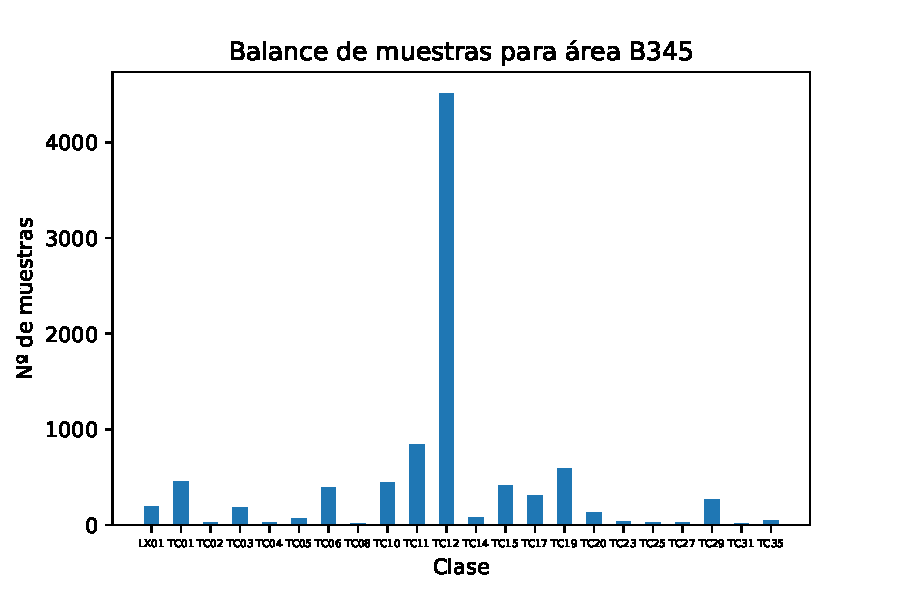
\includegraphics[width=\textwidth]{imagenes/resultados/balance/B345.pdf}
	\caption{Nº de muestras para el dataset del área B345}
	\label{fig:frecuencia_dataset_b345}
\end{figure}

\begin{table}[H]
	\centering
	\begin{tabular}{|c|c|}
		\hline
		Clase & Nº de muestras \\ \hline
		LX01 & 194 \\ \hline
		TC01 & 457 \\ \hline
		TC02 & 22 \\ \hline
		TC03 & 185 \\ \hline
		TC04 & 25 \\ \hline
		TC05 & 64 \\ \hline
		TC06 & 397 \\ \hline
		TC08 & 15 \\ \hline
		TC10 & 442 \\ \hline
		TC11 & 838 \\ \hline
		TC12 & 4511 \\ \hline
	\end{tabular}
	\begin{tabular}{|c|c|}
		\hline	
		TC14 & 82 \\ \hline
		TC15 & 414 \\ \hline
		TC17 & 304 \\ \hline
		TC19 & 590 \\ \hline
		TC20 & 131 \\ \hline
		TC23 & 38 \\ \hline
		TC25 & 30 \\ \hline
		TC27 & 21 \\ \hline
		TC29 & 269 \\ \hline
		TC31 & 18 \\ \hline
		TC35 & 52 \\ \hline
	\end{tabular}
	\caption{N$^\circ$ de muestras para área B345}	
	\label{tab:n_muestras_b345}
\end{table}

\begin{figure}[H]
	\centering
	\captionsetup{justification=centering}
	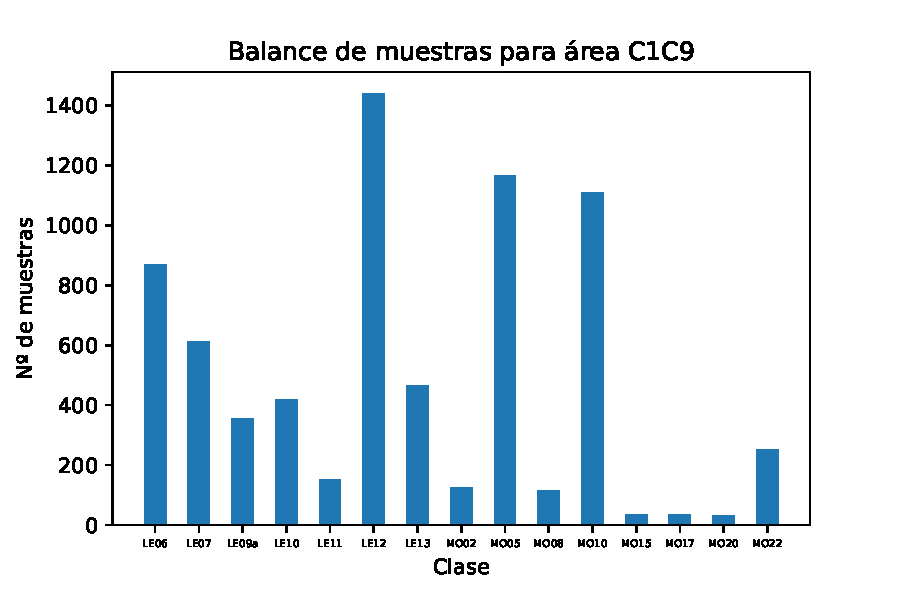
\includegraphics[width=\textwidth]{imagenes/resultados/balance/C1C9.pdf}
	\caption{Nº de muestras para el dataset del área C1C9}
	\label{fig:frecuencia_dataset_c1c9}
\end{figure}


\begin{table}[H]
	\centering
	\begin{tabular}{|c|c|}
		\hline
		Clase & Nº de muestras \\ \hline
		LE06 & 869 \\ \hline
		LE07 & 613 \\ \hline
		LE09a & 354 \\ \hline
		LE10 & 418 \\ \hline
		LE11 & 153 \\ \hline
		LE12 & 1440 \\ \hline
		LE13 & 464 \\ \hline
		MO02 & 124 \\ \hline
	\end{tabular}
	\begin{tabular}{|c|c|}
		\hline	
		MO05 & 1168 \\ \hline
		MO08 & 116 \\ \hline
		MO10 & 1109 \\ \hline
		MO15 & 35 \\ \hline
		MO17 & 34 \\ \hline
		MO20 & 31 \\ \hline
		MO22 & 253 \\ \hline
	\end{tabular}
	\caption{N$^\circ$ de muestras para área C1C9}	
	\label{tab:n_muestras_c1c9}
\end{table}

Para analizar resultados, al tratar con clases desbalanceadas, no se usa en ningún momento la exactitud y, a priori, tanto promedio micro, macro y ponderado de las métricas darán resultados que favorezcan a las clases más frecuentes.

\section{ANOVA}

El método LBP no ha sido utilizado debido a que el numero de características extraídas de una imagen depende de su resolución. Dado que el dataset contiene imágenes con resoluciones diferentes, no se puede obtener un número uniforme de características.

Para la selección de características con ANOVA, se obtienen los siguientes resultados:

\subsection{Área B345}

\begin{table}[H]
	\centering
	\begin{tabular}{|c|c|}
		\hline
		Característica & F-valor \\ \hline
		H0 & 23859.201619 \\ \hline
		H4 & 12429.265116 \\ \hline
		H6 & 7880.238366 \\ \hline
		M3 & 3895.946032 \\ \hline
		H1 & 3827.930644 \\ \hline
		M0 & 3486.251597 \\ \hline
		H5 & 3090.149390 \\ \hline
		M2 & 2880.764008 \\ \hline
		F7 & 2439.522794 \\ \hline
		F6 & 1810.805758 \\ \hline
		H2 & 1715.595292 \\ \hline
		F5 & 1267.176107 \\ \hline
		F4 & 1049.974086 \\ \hline
		M1 & 1003.760963 \\ \hline
		F2 & 879.120903 \\ \hline
	\end{tabular}
	\begin{tabular}{|c|c|}
		\hline
		F3 & 821.479145 \\ \hline
		F11 & 675.605577 \\ \hline
		F1 & 670.737686 \\ \hline
		F0 & 661.628967 \\ \hline
		M4 & 514.887416 \\ \hline
		F9 & 472.654444 \\ \hline
		M5 & 386.561602 \\ \hline
		F12 & 369.108364 \\ \hline
		M6 & 202.739105 \\ \hline
		F8 & 202.675900 \\ \hline
		F14 & 172.541408 \\ \hline
		F10 & 144.443042 \\ \hline
		F15 & 86.515230 \\ \hline
		F13 & 77.369423 \\ \hline
		H3 & nan \\ \hline
		H7 & nan \\ \hline
	\end{tabular}	
	\caption{Resultados ANOVA para área B345}	
	\label{tab:anova_b345}
\end{table}

\begin{figure}[H]
	\centering
	\captionsetup{justification=centering}
	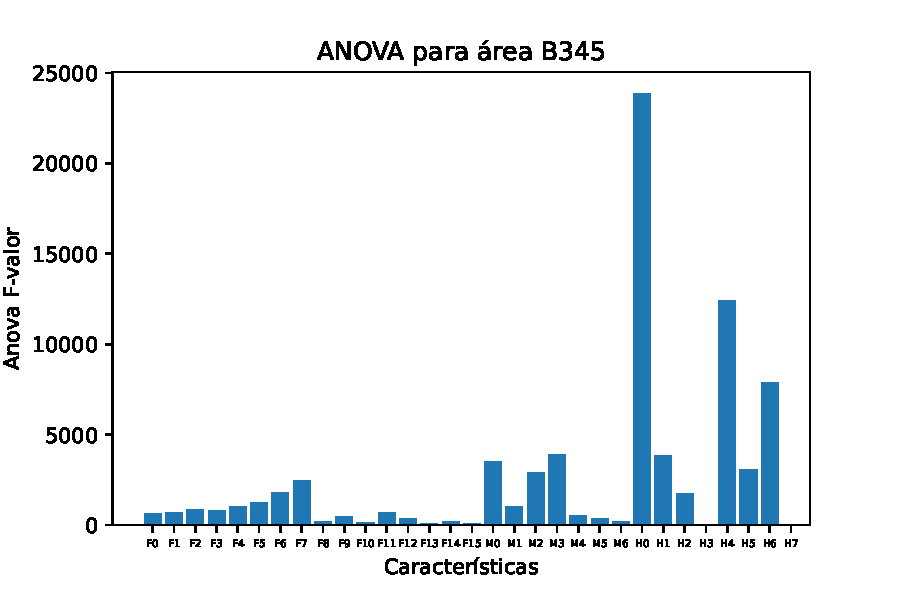
\includegraphics[width=\textwidth]{imagenes/resultados/anova/ANOVA_b345.pdf}
	\caption{Resultados ANOVA para área B345}
\end{figure}

De entre todas las características extraídas, por el método ANOVA se ha determinado que H0, H1, H4, H5, H6 y F7 son las seis características más discriminantes, seguidas por los momentos M0, M1, M2 y M3.

En el caso de H3 y H7, ANOVA devuelve un valor no definido pues, estas características son constantes para todas las muestras.

\subsection{Área C1C9}

\begin{table}[H]
	\begin{tabular}{|c|c|}
		\hline
		Característica & F-valor \\ \hline
		M1 & 6125.638894 \\ \hline
		H4 & 5857.112939 \\ \hline
		H0 & 4554.790583 \\ \hline
		M0 & 3048.724574 \\ \hline
		H5 & 1787.841543 \\ \hline
		M2 & 1752.153444 \\ \hline
		H2 & 1427.452251 \\ \hline
		H1 & 1040.217828 \\ \hline
		M3 & 817.966512 \\ \hline
		F3 & 528.279034 \\ \hline
		H6 & 376.474004 \\ \hline
		F7 & 276.076666 \\ \hline
		F1 & 267.434392 \\ \hline
		F10 & 252.051888 \\ \hline
		M5 & 229.500016 \\ \hline
	\end{tabular}	
	\begin{tabular}{|c|c|}
		\hline
		F6 & 221.004593 \\ \hline
		F5 & 189.035358 \\ \hline
		F8 & 164.096954 \\ \hline
		F14 & 156.956539 \\ \hline
		M4 & 140.206197 \\ \hline
		F2 & 133.046369 \\ \hline
		F9 & 122.262756 \\ \hline
		F11 & 105.074395 \\ \hline
		F0 & 78.174618 \\ \hline
		F4 & 77.091309 \\ \hline
		M6 & 75.595968 \\ \hline
		F15 & 73.126625 \\ \hline
		F12 & 60.370951 \\ \hline
		F13 & 48.366221 \\ \hline
		H3 & nan \\ \hline
		H7 & nan \\ \hline
	\end{tabular}	
	\caption{Resultados ANOVA para área C1C9}
	\label{tab:anova_c1c9}
\end{table}

\begin{figure}[H]
	\centering
	\captionsetup{justification=centering}
	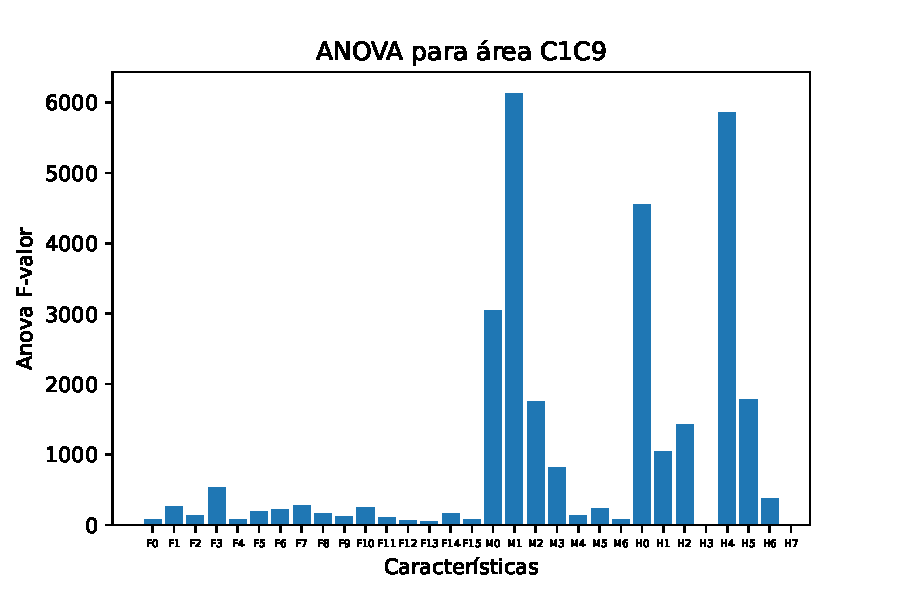
\includegraphics[width=\textwidth]{imagenes/resultados/anova/ANOVA_C1C9.pdf}
	\caption{Resultados ANOVA para área C1C9}
\end{figure}

Al igual que en el área B345, las características de Hog siguen siendo significativas, pero en este caso el momento de Hu segundo (M1) es la segunda característica más significativa.

Igual que para B345, H3 y H7 no están definidas ($NaN$) por ser constantes.

\mynote{Usando la clase \textit{SelectKBest}, proporcionada por Sklearn, se pueden escoger automáticamente las k mejores características según los F-valores de ANOVA.}

\section{K-vecinos más cercanos}

Al no devolver Knn predicciones probabilísticas, no se usa la curva ROC ó Precisión-Exhaustividad para analizar sus resultados.

\subsection{Resultados con clasificador Knn para área B345}

\subsubsection{Curvas de validación para Knn}

A continuación, se presenta la curva de validación para ambos modelos de clasificador Knn (uniforme y distancia) para las métricas de recall, precisión y $f_{1}$. 

Para todos los resultados, se han seleccionado las siete mejores características según ANOVA (véase \ref{tab:anova_b345}).

\begin{figure}[H]
	\centering
	\captionsetup{justification=centering}
	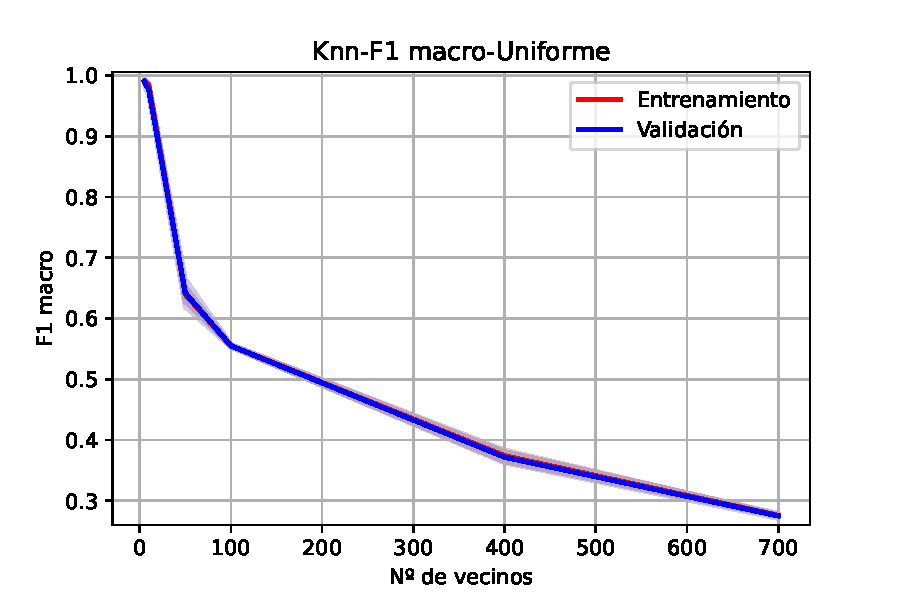
\includegraphics[width=\textwidth]{imagenes/resultados/curvas_validación/Knn-F1 macro-Uniforme.pdf}
	\caption{Curva de validación para modelo KNN uniforme, F1 macro}
	\label{fig:res_knn_vc_f1}
\end{figure}

\begin{figure}[H]
	\centering
	\captionsetup{justification=centering}
	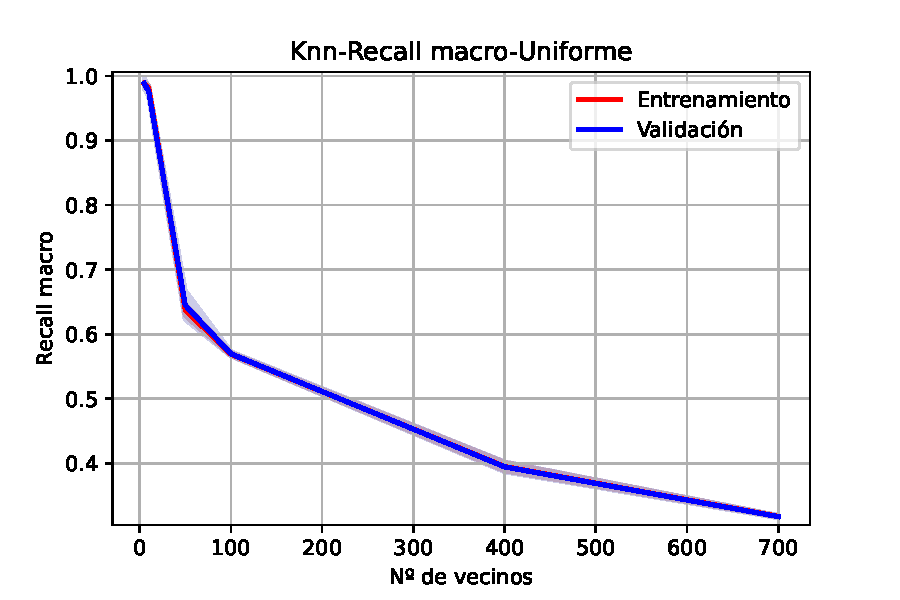
\includegraphics[width=\textwidth]{imagenes/resultados/curvas_validación/Knn-Recall macro-Uniforme.pdf}
	\caption{Curva de validación para modelo KNN uniforme, Recall macro}
	\label{fig:res_knn_vc_recall}
\end{figure}

\begin{figure}[H]
	\centering
	\captionsetup{justification=centering}
	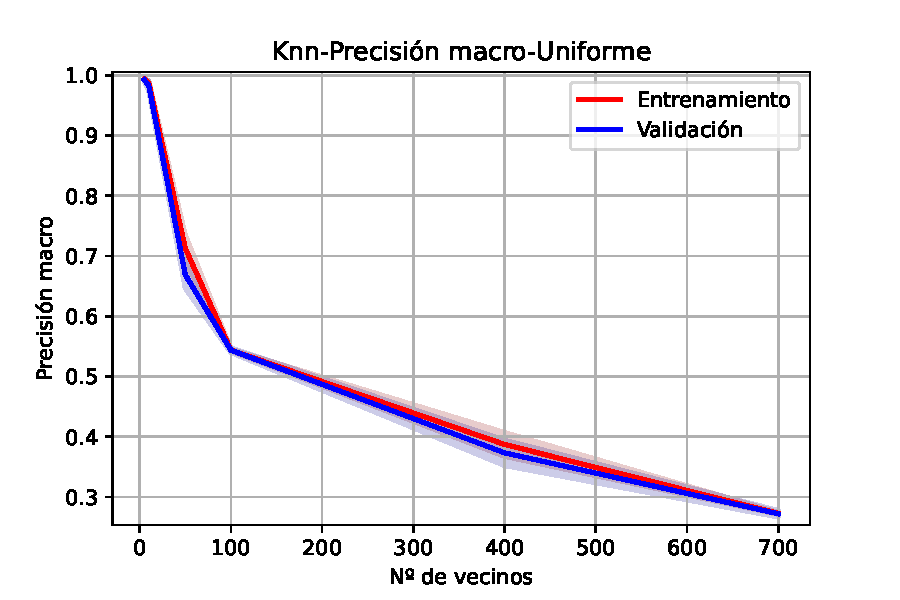
\includegraphics[width=\textwidth]{imagenes/resultados/curvas_validación/Knn-Precisión macro-Uniforme.pdf}
	\caption{Curva de validación para modelo KNN uniforme, Precisión macro}
	\label{fig:res_knn_vc_precision}
\end{figure}

Las tres figuras muestran la independencia del nº de vecinos del clasificador frente a un sobre ajuste y sub ajuste del modelo. También, para siete características, a mayor valores de $n$ peor es el resultado del modelo. 

Los mejores resultados se obtienen para el rango de $\left[5,20\right]$, como se muestra en las siguientes figuras:

\begin{figure}[H]
	\centering
	\captionsetup{justification=centering}
	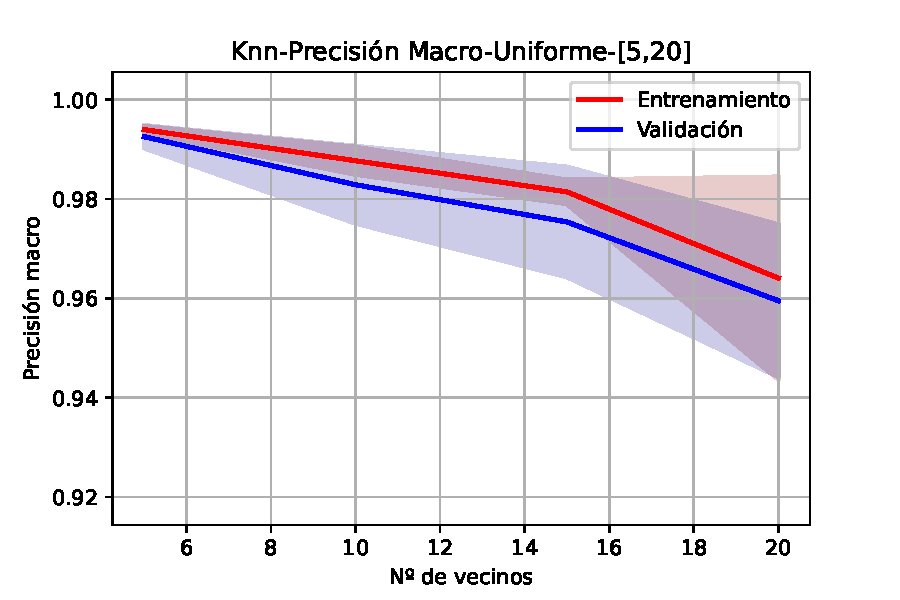
\includegraphics[width=\textwidth]{imagenes/resultados/curvas_validación/Knn-Precisión Macro-Uniforme-[5,20].pdf}
	\caption{Curva de validación para modelo KNN uniforme en rango n=[5,20], Precisión macro}
	\label{fig:res_knn_vc_precision_5,20}
\end{figure}

\begin{figure}[H]
	\centering
	\captionsetup{justification=centering}
	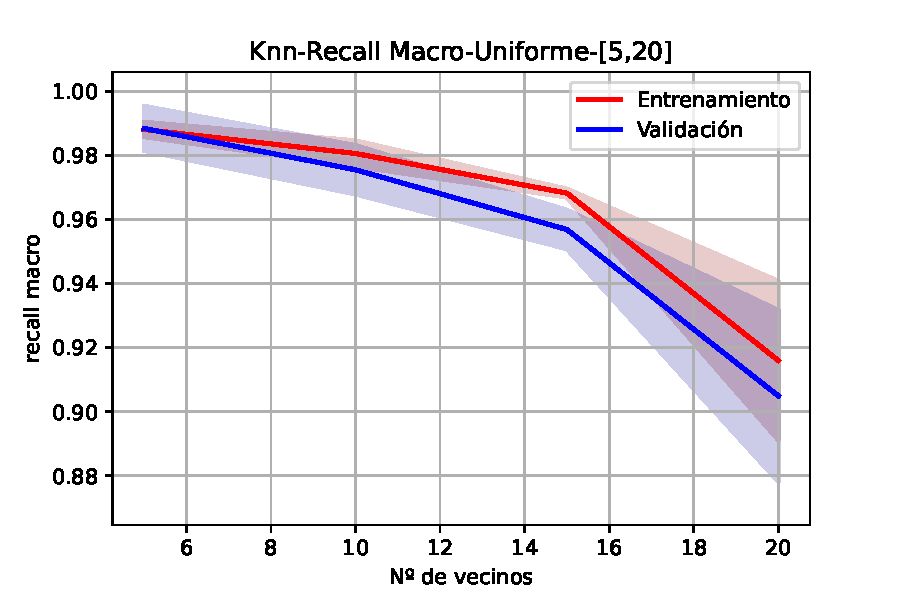
\includegraphics[width=\textwidth]{imagenes/resultados/curvas_validación/Knn-Recall Macro-Uniforme-[5,20].pdf}
	\caption{Curva de validación para modelo KNN uniforme en rango n=[5,20], Recall macro}
	\label{fig:res_knn_vc_recall_5,20}
\end{figure}

\begin{figure}[H]
	\centering
	\captionsetup{justification=centering}
	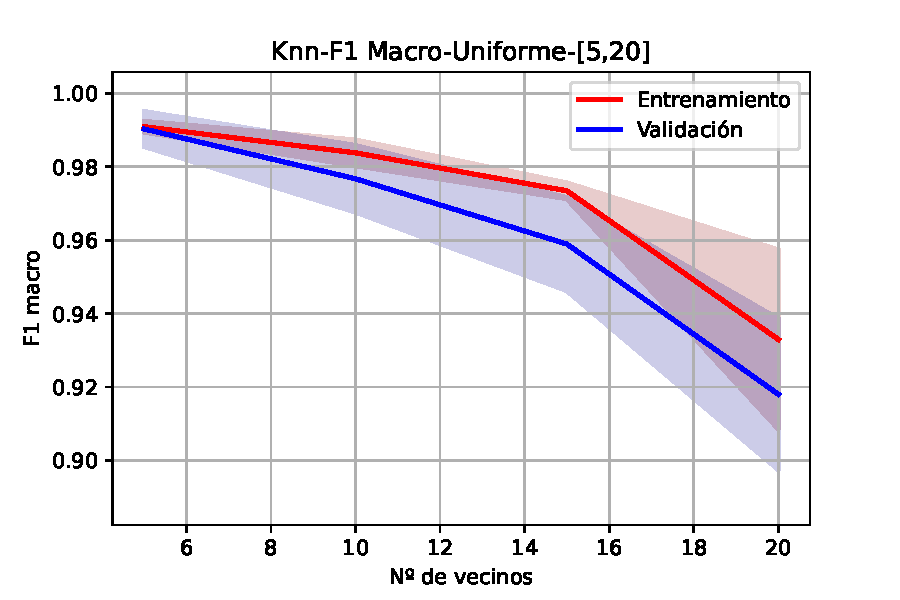
\includegraphics[width=\textwidth]{imagenes/resultados/curvas_validación/Knn-F1 Macro-Uniforme-[5,20].pdf}
	\caption{Curva de validación para modelo KNN uniforme en rango n=[5,20], F1 macro}
	\label{fig:res_knn_vc_f1_5,20}
\end{figure}

En todas las figuras, sobre todo \ref{fig:res_knn_vc_f1_5,20} y \ref{fig:res_knn_vc_recall_5,20}, a partir de $n=15$, inclusive, se presenta un aumento en la desviación de las métricas, indicando una mayor variación en el rendimiento en función de la partición escogida del dataset, lo que representa una menor capacidad de generalización del modelo en la fase de entrenamiento, que no consigue plasmar los mismos buenos resultados (en comparación, porque en general son excelentes, aún con este desliz) en la fase de validación.

De las seis figuras anteriores, se puede afirmar que los mejores resultados, con las siete mejores características, se dan para $n<15$.

\subsubsection{Mejores parámetros B345}

Realizando una búsqueda de parámetros entre $[2,31]$ mejores características y $[5,30]$ vecinos más cercanos, con una estrategia de validación cruzada y mezclado de datos, se obtiene la tabla \ref{res:knn_gs_b345}.

\begin{table}[H]
	\centering
	\captionsetup{justification=centering}
	\begin{tabular}{|c|c|}
		\hline
		Nº de características & 19 \\ \hline
		Nº de vecinos & 6 \\ \hline
	\end{tabular}
	\caption{Mejores parámetros modelo Knn para área B345}
	\label{res:knn_gs_b345}
\end{table}

Los resultados por clase y promediados para un modelo knn de 6 vecinos más cercanos utilizando las 19 mejores características devuelve los resultados de la tabla \ref{res:knn_report_b345}.

\begin{table}[H]
	\centering
	\captionsetup{justification=centering}
	\begin{tabular}{|c|c|c|c|c|}
		\hline
		\multicolumn{5}{|c|}{Métricas por clase} \\ \hline
		Clase & Precisión & Recall & F1 & Nº de muestras \\ \hline \hline
		LX01 & 1.000000 & 0.994845 & 0.997416 & 194 \\ \hline
		TC01 & 0.995643 & 1.000000 & 0.997817 & 457 \\ \hline
		TC02 & 1.000000 & 1.000000 & 1.000000 & 22 \\ \hline
		TC03 & 1.000000 & 1.000000 & 1.000000 & 185 \\ \hline
		TC04 & 1.000000 & 0.960000 & 0.979592 & 25 \\ \hline
		TC05 & 0.984615 & 1.000000 & 0.992248 & 64 \\ \hline
		TC06 & 1.000000 & 1.000000 & 1.000000 & 397 \\ \hline
		TC08 & 1.000000 & 0.933333 & 0.965517 & 15 \\ \hline
		TC10 & 0.972540 & 0.961538 & 0.967008 & 442 \\ \hline
		TC11 & 0.979834 & 0.985680 & 0.982748 & 838 \\ \hline
		TC12 & 0.999778 & 1.000000 & 0.999889 & 4511 \\ \hline
		TC14 & 1.000000 & 0.987805 & 0.993865 & 82 \\ \hline
		TC15 & 0.997590 & 1.000000 & 0.998794 & 414 \\ \hline
		TC17 & 0.996721 & 1.000000 & 0.998358 & 304 \\ \hline
		TC19 & 0.998305 & 0.998305 & 0.998305 & 590 \\ \hline
		TC20 & 0.992424 & 1.000000 & 0.996198 & 131 \\ \hline
		TC23 & 1.000000 & 0.921053 & 0.958904 & 38 \\ \hline
		TC25 & 1.000000 & 1.000000 & 1.000000 & 30 \\ \hline
		TC27 & 1.000000 & 1.000000 & 1.000000 & 21 \\ \hline
		TC29 & 1.000000 & 1.000000 & 1.000000 & 269 \\ \hline
		TC31 & 1.000000 & 1.000000 & 1.000000 & 18 \\ \hline
		TC35 & 1.000000 & 1.000000 & 1.000000 & 52 \\ \hline \hline
		Micro & 0.995934 & 0.995934 & 0.995934 & 9099 \\ \hline
		Macro & 0.952933 & 0.945329 & 0.948985 & 9099 \\ \hline
		Ponderada & 0.995934 & 0.995934 & 0.995920 & 9099 \\ \hline
	\end{tabular}
	\caption{Métricas por clase y promedios para área B345 con modelo Knn}
	\label{res:knn_report_b345}	
\end{table}

\begin{table}[H]	
	\centering
	\captionsetup{justification=centering}
	\begin{tabular}{|c|c|c|c|}
		\hline
		Promedio & Precisión & Recall & F1 \\ \hline
		Micro & 99.59\% & 99.59\% & 99.59\% \\ \hline
		Macro & 95.29\% & 94.53\% & 94.90\% \\ \hline
		Ponderada & 99.59\% & 99.59\% & 99.59\% \\ \hline
	\end{tabular}
	\caption{Métricas promediadas Knn B345}
	\label{res:knn_report_resumen_b345}
\end{table}

La tabla \ref{res:knn_report_resumen_b345} muestra que los resultados promedios para el problema general son muy elevados, obteniéndose un $94.9\%$ para $F_{1}$. La diferencia entre los promediados micro y ponderado frente al macro indican (además de un desbalanceado en los datos) que no todas las clases tienen un rendimiento cerca del $100\%$ como indicarían los otros promedios, la TC23 obtiene un $F_{1} = 95.89\%$ y sólo presenta 38 muestras, por ejemplo. Sin embargo, los resultados son más que satisfactorios dada la poca cantidad de muestras y la gran cantidad de clases (22). Los valores de recall y precisión indican que el modelo es bueno identificando muestras positivas de cada clase y acertando en la identificación de estas a la clase pertinente, respectivamente.

\mynote{Es muy posible que se obtengan resultados diferentes por milésimas seleccionando menos características, ya que el método \textit{GridSearchCV} va a buscar el mejor valor posible según la métrica escogida y devolverá los parámetros de esa métrica, sin considerar que el segundo mejor valor puede estar en el orden de millonésimas por debajo. Sin embargo, con los parámetros escogidos, la clasificación es la mejor posible, así que tampoco importa cuantos coja. Se puede jugar un poco y obtener la métrica para cada combinación de parámetros, pero no es el objetivo de este trabajo, solo decir que para estos parámetros el clasificador funciona que da gusto.}
	
%\subsubsection{Influencia del nº de características en el modelo Knn}
%\begin{table}[H]
%	\resizebox{\textwidth}{!}{
%	\begin{tabular}{|c|c|c|c|c|c|c|c|c|c|c|}
%		\hline
%		k/N & 5 & 6 & 7 & 8 & 9 & 10 & 11 & 12 & 13 & 15 \\ \hline
%		2 & 0.750197 & 0.732362 & 0.731626 & 0.718620 & 0.713603 & 0.706865 & 0.695101 & 0.664370 & 0.649346 & 0.636021 \\ \hline
%		3 & 0.846253 & 0.836495 & 0.842503 & 0.824873 & 0.829736 & 0.820059 & 0.816807 & 0.809634 & 0.804559 & 0.801296 \\ \hline
%		4 & 0.901158 & 0.899806 & 0.895775 & 0.887616 & 0.885607 & 0.879149 & 0.876432 & 0.858412 & 0.854349 & 0.847261 \\ \hline
%		5 & 0.981725 & 0.979560 & 0.972743 & 0.964084 & 0.963459 & 0.956822 & 0.954959 & 0.945003 & 0.945325 & 0.930744 \\ \hline
%		6 & 0.987181 & 0.981166 & 0.973448 & 0.963671 & 0.963409 & 0.956422 & 0.942576 & 0.941990 & 0.939666 & 0.935943 \\ \hline
%		7 & 0.988256 & 0.985800 & 0.981250 & 0.979446 & 0.976043 & 0.973633 & 0.972225 & 0.962696 & 0.958911 & 0.957556 \\ \hline
%		8 & 0.987228 & 0.979825 & 0.979331 & 0.975007 & 0.974665 & 0.969068 & 0.968959 & 0.966239 & 0.966950 & 0.955709 \\ \hline
%		9 & 0.986717 & 0.984970 & 0.984872 & 0.978443 & 0.978988 & 0.971343 & 0.971098 & 0.964389 & 0.964831 & 0.953251 \\ \hline
%		10 & 0.988313 & 0.983662 & 0.984488 & 0.976018 & 0.976452 & 0.974554 & 0.974404 & 0.968801 & 0.969779 & 0.964441 \\ \hline
%		11 & 0.985269 & 0.983850 & 0.984471 & 0.981281 & 0.981639 & 0.977377 & 0.978565 & 0.969286 & 0.969621 & 0.960472 \\ \hline
%		12 & 0.989227 & 0.986803 & 0.986217 & 0.985610 & 0.985447 & 0.982737 & 0.982819 & 0.975377 & 0.974679 & 0.965164 \\ \hline
%		13 & 0.991577 & 0.988773 & 0.987402 & 0.983631 & 0.985323 & 0.978803 & 0.978720 & 0.965096 & 0.966117 & 0.959325 \\ \hline
%		15 & 0.991461 & 0.985820 & 0.985076 & 0.984702 & 0.984453 & 0.982741 & 0.983352 & 0.979010 & 0.978615 & 0.969601 \\ \hline
%	\end{tabular}}
%	\caption{F1 macro para diferentes N\textdegree de vecinos en función del número de mejores características}
%	\label{tab:res_knn_kvsn}
%\end{table}
%
%\mynote{En la tabla \ref{tab:res_knn_kvsn} solo se muestran quince de las treinta y una características pues, además del tamaño considerable de la tabla en la página, a partir de 16 $F_{1}$ sólo aumenta en milésimas. La tabla completa se encuentra en los anexos de resultados.}
%
%En la tabla \ref{tab:res_knn_kvsn}, a partir de 5 características $F_{1}$ se estabiliza, aumentando su valor 1-2 décimas (2-3 para mayores valores de N)
%hasta llegar a las 15 características. Además, según la tabla \ref{tab:res_knn_kvsn_stdev}, a mayor valor de k menor es la desviación de la métrica.
%
%Por tanto, se puede concluir que cualquier valor de $n$ en el rango [5,15) presenta buenos resultados para el área B345.
%
%\begin{table}[H]
%	\resizebox{\textwidth}{!}{
%	\begin{tabular}{|c|c|c|c|c|c|c|c|c|c|c|}
%		\hline
%		k/N & 5 & 6 & 7 & 8 & 9 & 10 & 11 & 12 & 13 & 15 \\ \hline
%		2 & 0.031263 & 0.028918 & 0.027425 & 0.038645 & 0.038485 & 0.033838 & 0.027380 & 0.011099 & 0.011499 & 0.019158 \\ \hline
%		3 & 0.022516 & 0.023287 & 0.021248 & 0.020090 & 0.021299 & 0.014314 & 0.012023 & 0.013558 & 0.016777 & 0.015160 \\ \hline
%		4 & 0.011580 & 0.010484 & 0.013045 & 0.013121 & 0.014088 & 0.018962 & 0.020212 & 0.006876 & 0.011304 & 0.013484 \\ \hline
%		5 & 0.007101 & 0.008787 & 0.015885 & 0.017089 & 0.017825 & 0.018747 & 0.015785 & 0.016174 & 0.016110 & 0.013600 \\ \hline
%		6 & 0.009172 & 0.011432 & 0.008986 & 0.018212 & 0.016982 & 0.017263 & 0.017706 & 0.018679 & 0.015959 & 0.014962 \\ \hline
%		7 & 0.004283 & 0.005415 & 0.007737 & 0.007010 & 0.015303 & 0.013305 & 0.014690 & 0.017637 & 0.015151 & 0.014291 \\ \hline
%		8 & 0.001790 & 0.010028 & 0.010619 & 0.009653 & 0.010005 & 0.011424 & 0.011686 & 0.012188 & 0.012579 & 0.017748 \\ \hline
%		9 & 0.004908 & 0.004796 & 0.004699 & 0.008346 & 0.008339 & 0.008184 & 0.008223 & 0.011039 & 0.010391 & 0.008906 \\ \hline
%		10 & 0.005957 & 0.007101 & 0.007109 & 0.012818 & 0.012815 & 0.013961 & 0.014291 & 0.015866 & 0.016634 & 0.013791 \\ \hline
%		11 & 0.012960 & 0.013744 & 0.013643 & 0.012318 & 0.014393 & 0.013041 & 0.013674 & 0.015642 & 0.015421 & 0.022719 \\ \hline
%		12 & 0.004536 & 0.003496 & 0.003331 & 0.003176 & 0.002955 & 0.002077 & 0.002331 & 0.005933 & 0.007653 & 0.008392 \\ \hline
%		13 & 0.003761 & 0.004431 & 0.004382 & 0.005867 & 0.007458 & 0.008414 & 0.008670 & 0.018212 & 0.018673 & 0.015392 \\ \hline
%		15 & 0.004415 & 0.009609 & 0.009790 & 0.009930 & 0.009757 & 0.011447 & 0.010203 & 0.009231 & 0.009019 & 0.015241 \\ \hline
%	\end{tabular}}
%	\caption{Desviación típica para tabla superior.}
%	\label{tab:res_knn_kvsn_stdev}
%\end{table}
%
%\begin{figure}[H]
%	\centering
%	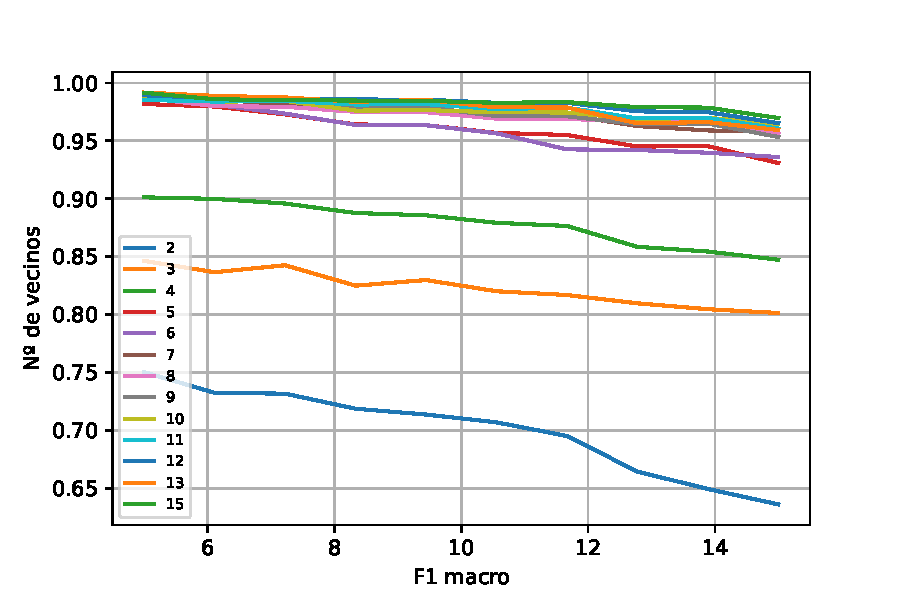
\includegraphics[width=\textwidth]{imagenes/resultados/knn/knn_f1vsn.pdf}
%	\caption{F1 macro en función del nº de vecinos para modelo Knn}
%	\label{res:knn_f1vsn}
%\end{figure}
%
%
%\begin{table}[H]
%	\centering
%	\begin{tabular}{|c|c|c|c|c|}
%		\hline
%		\multicolumn{5}{|c|}{Métricas por clase} \\ \hline
%		Clase & Precisión & Recall & F1 & Nº de muestras \\ \hline \hline
%		LX01 & 0.994792 & 0.984536 & 0.989637 & 194 \\ \hline
%		TC01 & 0.995643 & 1.000000 & 0.997817 & 457 \\ \hline
%		TC02 & 0.956522 & 1.000000 & 0.977778 & 22 \\ \hline
%		TC03 & 1.000000 & 0.994595 & 0.997290 & 185 \\ \hline
%		TC04 & 1.000000 & 0.960000 & 0.979592 & 25 \\ \hline
%		TC05 & 0.984615 & 1.000000 & 0.992248 & 64 \\ \hline
%		TC06 & 1.000000 & 0.997481 & 0.998739 & 397 \\ \hline
%		TC08 & 1.000000 & 1.000000 & 1.000000 & 15 \\ \hline
%		TC10 & 0.909292 & 0.929864 & 0.919463 & 442 \\ \hline
%		TC11 & 0.962740 & 0.955847 & 0.959281 & 838 \\ \hline
%		TC12 & 0.999335 & 1.000000 & 0.999668 & 4511 \\ \hline
%		TC14 & 1.000000 & 0.987805 & 0.993865 & 82 \\ \hline
%		TC15 & 0.997585 & 0.997585 & 0.997585 & 414 \\ \hline
%		TC17 & 0.986928 & 0.993421 & 0.990164 & 304 \\ \hline
%		TC19 & 1.000000 & 0.998305 & 0.999152 & 590 \\ \hline
%		TC20 & 0.992424 & 1.000000 & 0.996198 & 131 \\ \hline
%		TC23 & 1.000000 & 0.921053 & 0.958904 & 38 \\ \hline
%		TC25 & 1.000000 & 0.933333 & 0.965517 & 30 \\ \hline
%		TC27 & 1.000000 & 0.904762 & 0.950000 & 21 \\ \hline
%		TC29 & 0.977695 & 0.977695 & 0.977695 & 269 \\ \hline
%		TC31 & 0.894737 & 0.944444 & 0.918919 & 18 \\ \hline
%		TC35 & 0.941176 & 0.923077 & 0.932039 & 52 \\ \hline \hline
%		Micro & 0.989339 & 0.989339 & 0.989339 & 9099 \\ \hline
%		Macro & 0.938847 & 0.930600 & 0.934415 & 9099 \\ \hline
%		Ponderada & 0.989430 & 0.989339 & 0.989355 & 9099 \\ \hline
%	\end{tabular}
%	\caption{Métricas para clases del área B345, con promedios}
%	\label{res:knn_class_report}
%\end{table}

\subsection{Resultados con clasificador Knn para área C1C9}

\subsubsection{Curvas de validación}

\begin{figure}[H]
	\centering
	\captionsetup{justification=centering}
	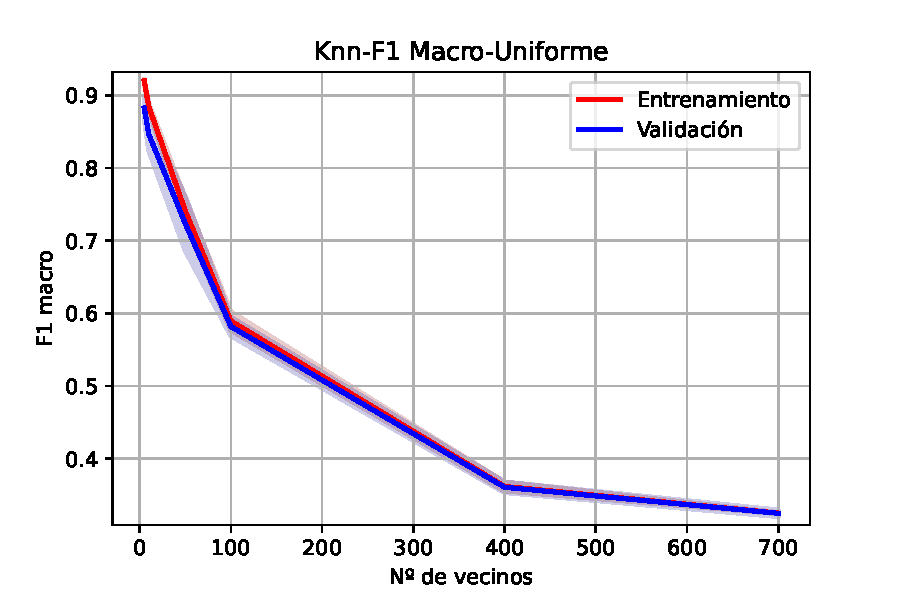
\includegraphics[width=\textwidth]{imagenes/resultados/curvas_validación/Knn-F1 macro-Uniforme-c1c9.pdf}
	\caption{Curva de validación para modelo KNN uniforme, F1 macro}
	\label{fig:res_knn_vc_f1_c1c9}
\end{figure}

\begin{figure}[H]
	\centering
	\captionsetup{justification=centering}
	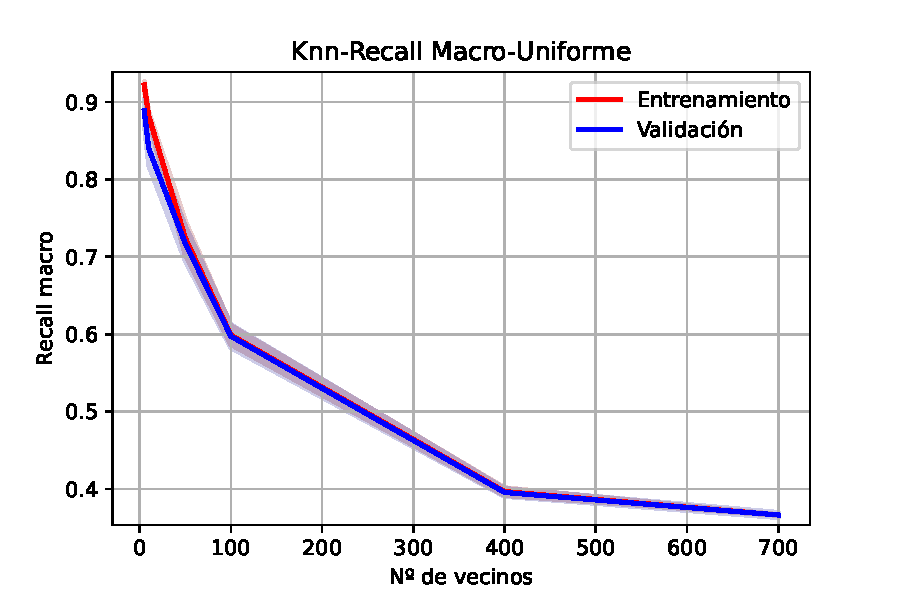
\includegraphics[width=\textwidth]{imagenes/resultados/curvas_validación/Knn-Recall macro-Uniforme-c1c9.pdf}
	\caption{Curva de validación para modelo KNN uniforme, Recall macro}
	\label{fig:res_knn_vc_recall_c1c9}
\end{figure}

\begin{figure}[H]
	\centering
	\captionsetup{justification=centering}
	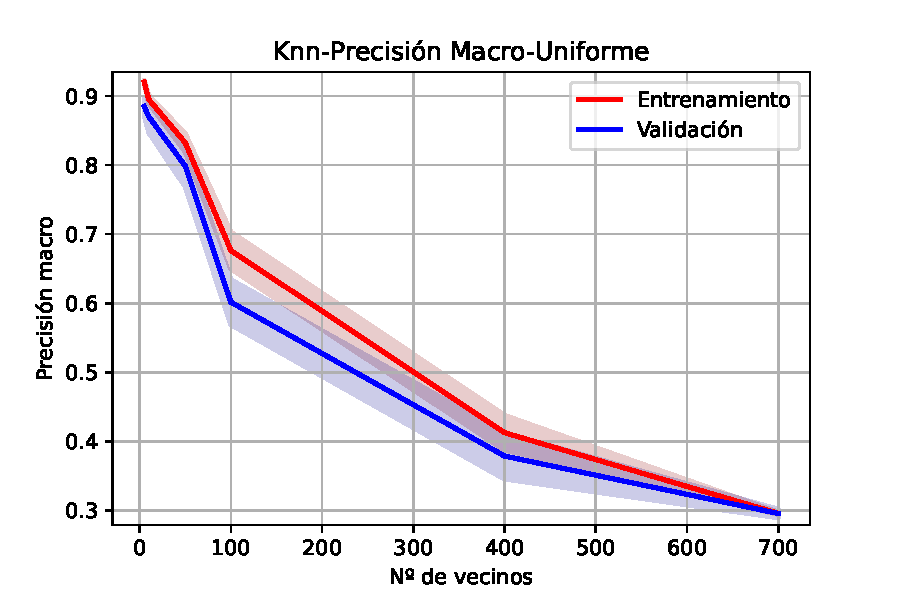
\includegraphics[width=\textwidth]{imagenes/resultados/curvas_validación/Knn-Precisión macro-Uniforme-c1c9.pdf}
	\caption{Curva de validación para modelo KNN uniforme, Precisión macro}
	\label{fig:res_knn_vc_precision_c1c9}
\end{figure}

A diferencia que para el área B345, en este caso la curva de validación para el área C1C9 muestra un resultado sobre ajustado en precisión. Aunque el modelo es exhaustivo encontrando muestras positivas, no consigue acertarlas correctamente. Los falsos positivos para el caso de validación son mayores que en el entrenamiento, indicando que existe una similitud entre varios símbolos que el clasificador no es capaz de discriminar correctamente. Este comportamiento se acentúa en $n=100$, desapareciendo por completo en $n=700$ y, aun así, los resultados son aceptables para $n<30$.

\begin{figure}[H]
	\centering
	\captionsetup{justification=centering}
	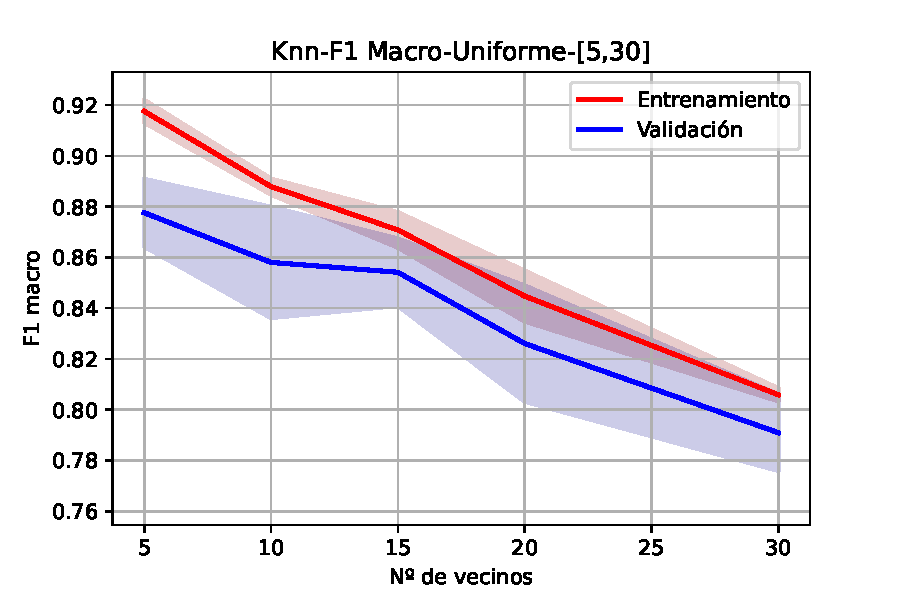
\includegraphics[width=\textwidth]{imagenes/resultados/curvas_validación/Knn-F1 Macro-Uniforme-c1c9[5,30].pdf}
	\caption{Curva de validación para modelo KNN uniforme, F1 macro}
	\label{fig:res_knn_vc_precision_c1c9[5,30]}
\end{figure}

\subsubsection{Mejores parámetros C1C9}

Realizando una búsqueda de parámetros entre $[2,31]$ mejores características y $[5,30]$ vecinos más cercanos, con una estrategia de validación cruzada y mezclado de datos, se obtiene la tabla \ref{res:knn_gs_c1c9}.

\begin{table}[H]
	\centering
	\captionsetup{justification=centering}
	\begin{tabular}{|c|c|}
		\hline
		Nº de características & 7 \\ \hline
		Nº de vecinos & 5 \\ \hline
	\end{tabular}
	\caption{Mejores parámetros modelo Knn para área C1C9}
	\label{res:knn_gs_c1c9}
\end{table}

Los resultados por clase y promediados para un modelo knn de 5 vecinos más cercanos utilizando las 7 mejores características devuelve los resultados de la tabla \ref{res:knn_report_c1c9}.

\begin{table}[H]
	\centering
	\captionsetup{justification=centering}
	\begin{tabular}{|c|c|c|c|c|}
		\hline
		\multicolumn{5}{|c|}{Métricas por clase} \\ \hline
		Clase & Precisión & Recall & F1 & Nº de muestras \\ \hline \hline
		LE06 & 0.794737 & 0.868815 & 0.830126 & 869 \\ \hline
		LE07 & 0.758879 & 0.662316 & 0.707317 & 613 \\ \hline
		LE09a & 0.991525 & 0.991525 & 0.991525 & 354 \\ \hline
		LE10 & 0.917040 & 0.978469 & 0.946759 & 418 \\ \hline
		LE11 & 0.888112 & 0.830065 & 0.858108 & 153 \\ \hline
		LE12 & 0.930061 & 0.960417 & 0.944995 & 1440 \\ \hline
		LE13 & 0.852217 & 0.745690 & 0.795402 & 464 \\ \hline
		MO02 & 0.881890 & 0.903226 & 0.892430 & 124 \\ \hline
		MO05 & 0.992201 & 0.980308 & 0.986219 & 1168 \\ \hline
		MO08 & 0.935185 & 0.870690 & 0.901786 & 116 \\ \hline
		MO10 & 0.956289 & 0.966637 & 0.961435 & 1109 \\ \hline
		MO15 & 0.842105 & 0.914286 & 0.876712 & 35 \\ \hline
		MO17 & 0.969697 & 0.941176 & 0.955224 & 34 \\ \hline
		MO20 & 0.658537 & 0.870968 & 0.750000 & 31 \\ \hline
		MO22 & 0.890756 & 0.837945 & 0.863544 & 253 \\ \hline
		Micro & 0.906559 & 0.906559 & 0.906559 & 7181 \\ \hline
		Macro & 0.576488 & 0.579241 & 0.576591 & 7181 \\ \hline
		Ponderada & 0.906031 & 0.906559 & 0.905327 & 7181 \\ \hline
	\end{tabular}
	\caption{Métricas por clase y promedios para área C1C9 con modelo Knn}
	\label{res:knn_report_c1c9}	
\end{table}

\begin{table}[H]	
	\centering
	\captionsetup{justification=centering}
	\begin{tabular}{|c|c|c|c|}
		\hline
		Promedio & Precisión & Recall & F1 \\ \hline
		Micro & 90.66\% & 90.66\% & 90.66\% \\ \hline
		Macro & 57.65\% & 57.92\% & 57.66\% \\ \hline
		Ponderada & 90.6\% & 90.66\% & 90.53\% \\ \hline
	\end{tabular}
	\caption{Métricas promediadas Knn C1C9}
	\label{res:knn_report_resumen_c1c9}
\end{table}

Las métricas ponderadas de la tabla \ref{res:knn_report_resumen_c1c9} revelan que, en el caso de promedio macro, aun existiendo clases con un alto valor de rendimiento, existen otras cuyos valores no son tal elevados, siendo aquellas menos frecuentes en el dataset. En general los resultados son aceptables, excepto para las clases MO20 y LE07.

\mynote{\textbf{Esto se debe a que la calidad de las imágenes de la C1C9 es bastante peor que la B345, porque en muchas aparecen hasta dedos. No sé si puedo mostrar imágenes ejemplo de los símbolos, pero supongo que si no, al menos puedo hacer un inciso a porqué los resultados salen peor que para la B345}.}

%\subsubsection{Influencia del nº de características en el modelo Knn}
%\begin{table}[H]
%	\resizebox{\textwidth}{!}{
%		\begin{tabular}{|c|c|c|c|c|c|c|c|c|c|c|}
%			\hline
%			k/n & 5 & 6 & 7 & 8 & 9 & 10 & 11 & 12 & 13 & 15 \\ \hline
%			2 & 0.660351 & 0.659113 & 0.649249 & 0.644123 & 0.652822 & 0.639869 & 0.655416 & 0.653679 & 0.637519 & 0.634175 \\ \hline
%			3 & 0.774633 & 0.764143 & 0.761893 & 0.754922 & 0.758031 & 0.754958 & 0.751379 & 0.743985 & 0.744765 & 0.740667 \\ \hline
%			4 & 0.834093 & 0.829328 & 0.829576 & 0.823813 & 0.822685 & 0.811232 & 0.808611 & 0.801191 & 0.805684 & 0.804415 \\ \hline
%			5 & 0.881294 & 0.871179 & 0.871143 & 0.869219 & 0.866350 & 0.866916 & 0.864499 & 0.856663 & 0.857033 & 0.857363 \\ \hline
%			6 & 0.876549 & 0.866209 & 0.872498 & 0.859462 & 0.858577 & 0.852567 & 0.851383 & 0.844738 & 0.847902 & 0.840928 \\ \hline
%			7 & 0.877466 & 0.864204 & 0.872170 & 0.861328 & 0.865580 & 0.858739 & 0.860466 & 0.849003 & 0.850871 & 0.842538 \\ \hline
%			8 & 0.881931 & 0.872454 & 0.878042 & 0.872454 & 0.871443 & 0.862174 & 0.868691 & 0.862320 & 0.863260 & 0.854792 \\ \hline
%			9 & 0.875723 & 0.861127 & 0.872371 & 0.858797 & 0.865442 & 0.852997 & 0.858776 & 0.844760 & 0.845437 & 0.838170 \\ \hline
%			10 & 0.880983 & 0.878961 & 0.872075 & 0.872905 & 0.866851 & 0.861961 & 0.860365 & 0.850296 & 0.847008 & 0.839249 \\ \hline
%			11 & 0.880941 & 0.871367 & 0.871894 & 0.867910 & 0.872122 & 0.862643 & 0.863072 & 0.855191 & 0.859294 & 0.846094 \\ \hline
%			12 & 0.884365 & 0.867537 & 0.873713 & 0.867695 & 0.865381 & 0.853263 & 0.859611 & 0.850419 & 0.852613 & 0.842012 \\ \hline
%			13 & 0.871192 & 0.857921 & 0.866745 & 0.854738 & 0.862419 & 0.853122 & 0.852007 & 0.848010 & 0.846950 & 0.837385 \\ \hline
%			14 & 0.867074 & 0.862574 & 0.868024 & 0.862102 & 0.863141 & 0.849403 & 0.854475 & 0.847440 & 0.848595 & 0.840671 \\ \hline
%			15 & 0.854392 & 0.843811 & 0.843492 & 0.829945 & 0.835355 & 0.809559 & 0.813387 & 0.801150 & 0.804072 & 0.794957 \\ \hline
%			16 & 0.856922 & 0.840174 & 0.847410 & 0.829957 & 0.826216 & 0.812471 & 0.812454 & 0.789768 & 0.807726 & 0.796728 \\ \hline
%			17 & 0.858164 & 0.845579 & 0.846955 & 0.833529 & 0.836478 & 0.818352 & 0.825421 & 0.812664 & 0.813273 & 0.800794 \\ \hline
%			18 & 0.854830 & 0.842250 & 0.838757 & 0.824953 & 0.821445 & 0.805324 & 0.813603 & 0.805735 & 0.802046 & 0.798083 \\ \hline
%			19 & 0.859329 & 0.840790 & 0.847554 & 0.836103 & 0.827789 & 0.811015 & 0.808460 & 0.798256 & 0.810436 & 0.797352 \\ \hline
%			20 & 0.835959 & 0.830450 & 0.833114 & 0.816145 & 0.809001 & 0.799138 & 0.787499 & 0.779040 & 0.775196 & 0.753221 \\ \hline
%			21 & 0.848853 & 0.817713 & 0.825867 & 0.814144 & 0.812350 & 0.804573 & 0.797692 & 0.778039 & 0.775528 & 0.765795 \\ \hline
%			22 & 0.836096 & 0.817077 & 0.824121 & 0.806797 & 0.803234 & 0.790651 & 0.782546 & 0.769489 & 0.761104 & 0.748714 \\ \hline
%			23 & 0.839378 & 0.822893 & 0.822122 & 0.813259 & 0.803920 & 0.789965 & 0.789334 & 0.765730 & 0.762785 & 0.753235 \\ \hline
%			24 & 0.852524 & 0.836858 & 0.834629 & 0.826161 & 0.815779 & 0.789310 & 0.773577 & 0.767940 & 0.764457 & 0.752308 \\ \hline
%			25 & 0.860073 & 0.841441 & 0.844501 & 0.823069 & 0.823015 & 0.805952 & 0.785418 & 0.772661 & 0.768648 & 0.752512 \\ \hline
%			26 & 0.835819 & 0.826877 & 0.823908 & 0.796692 & 0.791323 & 0.786089 & 0.777135 & 0.753200 & 0.742657 & 0.736103 \\ \hline
%			27 & 0.817487 & 0.807374 & 0.790659 & 0.782090 & 0.779622 & 0.763147 & 0.758142 & 0.740285 & 0.734570 & 0.728442 \\ \hline
%			28 & 0.836409 & 0.825019 & 0.820146 & 0.801469 & 0.798138 & 0.777125 & 0.774338 & 0.755973 & 0.752267 & 0.734691 \\ \hline
%			29 & 0.833154 & 0.825340 & 0.817927 & 0.805052 & 0.795270 & 0.779908 & 0.772263 & 0.752701 & 0.748578 & 0.737149 \\ \hline
%			31 & 0.822426 & 0.814392 & 0.818956 & 0.811287 & 0.813079 & 0.801768 & 0.794864 & 0.771089 & 0.756721 & 0.739770 \\ \hline
%	\end{tabular}}
%	\caption{F1 macro para diferentes N\textdegree de vecinos en función del número de mejores características}
%	\label{tab:res_knn_kvsn_c1c9}
%\end{table}

\section{SVM}

Los modelos SVM de \textit{Sklearn} permiten obtener predicciones probabilísticas de los datos de validación, permitiendo el uso de la curva de precisión-recall en la evaluación de su rendimiento.

\subsection{SVM con área C1c9}

\subsubsection{Curvas de validación para diferentes Kernel}

La cuadrícula de imágenes \ref{res:svc_vc} representa las curvas de validación para los diferentes kernel aplicables a un modelo SVM, implementados en la clase SVC de \textit{Sklearn}, definidos en las ecuaciones \ref{eqn:svm_kernel_lineal}, \ref{eqn:svm_kernel_rbf}, \ref{eqn:svm_kernel_poly} y \ref{eqn:svm_kernel_sigmoid}.

\begin{figure}[H]
	\captionsetup{justification=centering}
	\centering
	\begin{subfigure}[b]{.45\linewidth}
		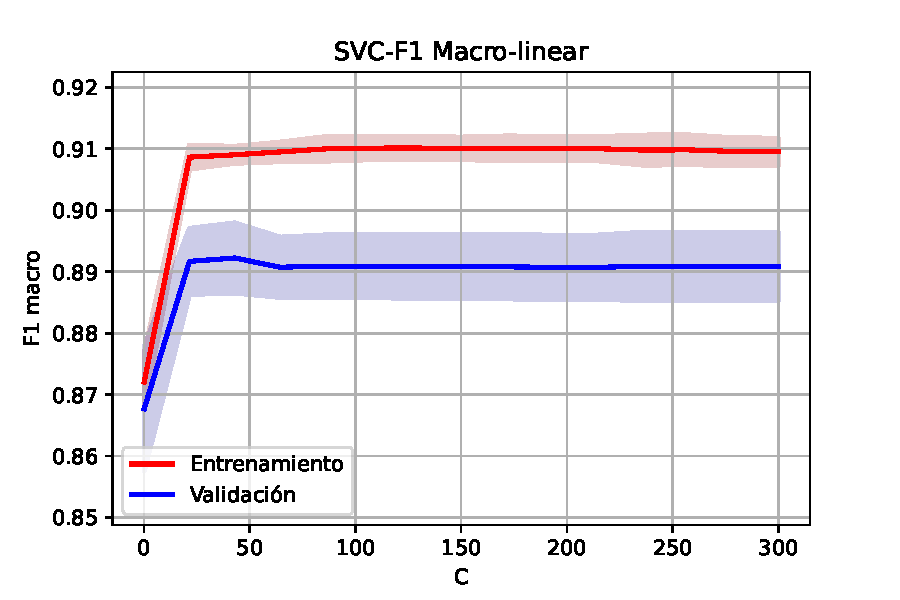
\includegraphics[width=\linewidth]{imagenes/resultados/svm/curvas_validacion/SVC-F1 Macro-linear.pdf}
		\caption{Kernel Lineal}
		\label{res:svc_vc_lineal}
	\end{subfigure}
	\begin{subfigure}[b]{.45\linewidth}
		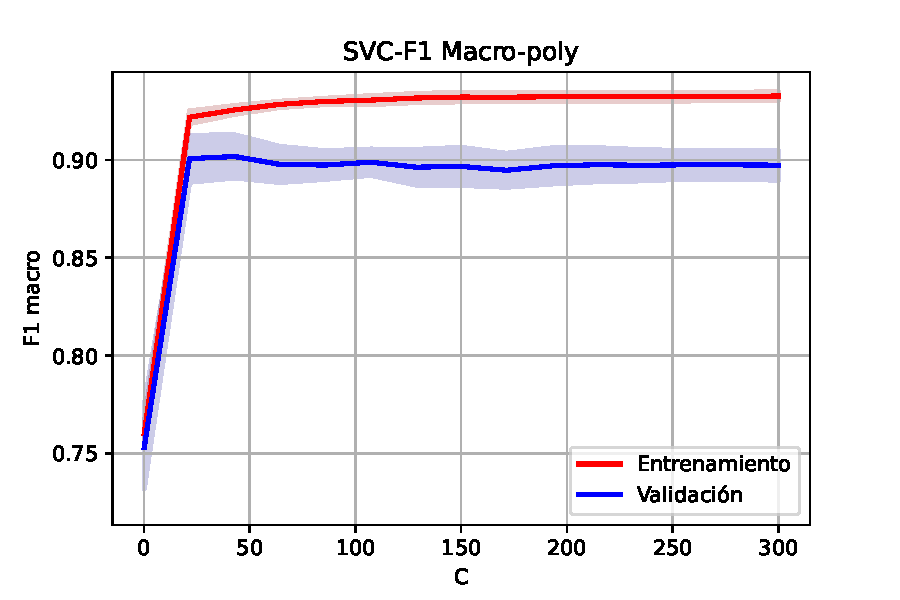
\includegraphics[width=\linewidth]{imagenes/resultados/svm/curvas_validacion/SVC-F1 Macro-poly.pdf}
		\caption{Kernel polinómico}
		\label{res:svc_vc_poly}
	\end{subfigure}
	\begin{subfigure}[b]{.45\linewidth}
		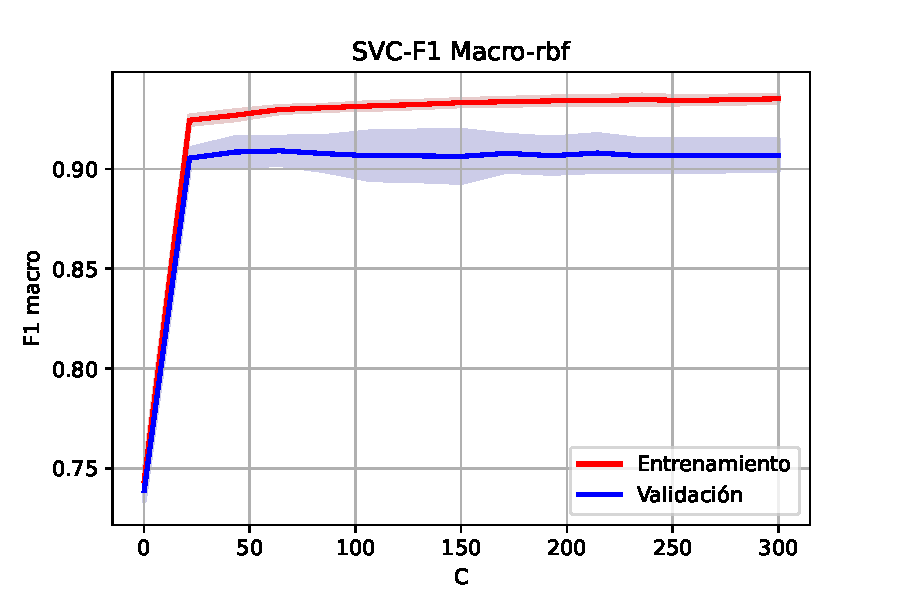
\includegraphics[width=\linewidth]{imagenes/resultados/svm/curvas_validacion/SVC-F1 Macro-rbf.pdf}
		\caption{Kernel RBF}
		\label{res:svc_vc_rbf}
	\end{subfigure}
	\begin{subfigure}[b]{.45\linewidth}
		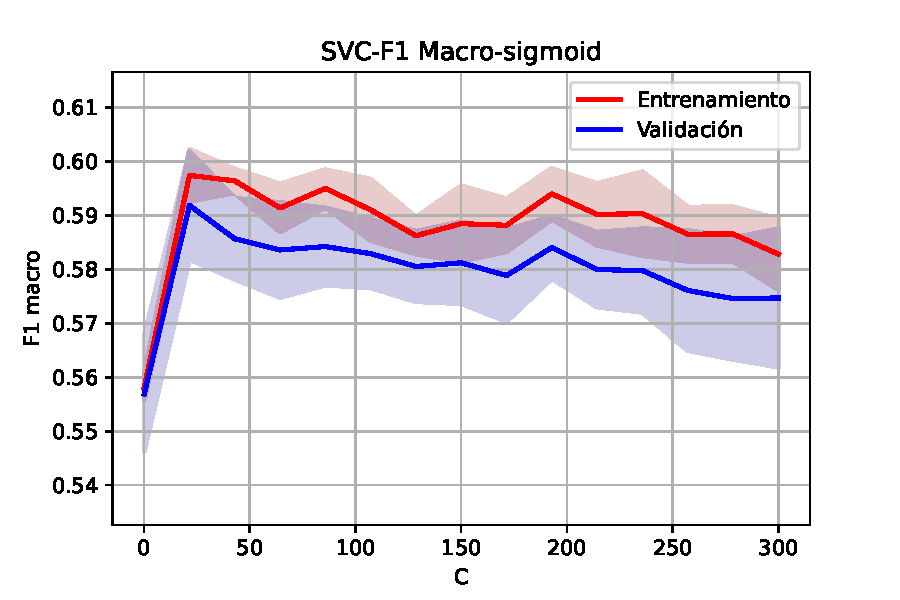
\includegraphics[width=\linewidth]{imagenes/resultados/svm/curvas_validacion/SVC-F1 Macro-sigmoid.pdf}
		\caption{Kernel Sigmoid}
		\label{res:svc_vc_sigmoid}
	\end{subfigure}
	\caption{Curvas de validación para kernels de modelo SVC en área C1c9 en función de parámetro de penalización C.}
	\label{res:svc_vc}
\end{figure}

Para los cuatro kernel disponibles en la clase SVC de \textit{Sklearn}, el modelo presenta para valores altos de C un sobreajuste de los datos de entrenamiento frente a los de validación. Para valores pequeños de C, el modelo tiene un buen comportamiento.

La figura \ref{res:svc_vc_sigmoid} presenta un rendimiento inferior a 0.6, indicando que el kernel \textit{sigmoid} no es aplicable a esta clasificación.

\paragraph{Kernel RBF}

El kernel RBF (ecuación \ref{eqn:svm_kernel_rbf}) depende del parámetro $\gamma$ en su definición. La figura \ref{res:svc_vc_rbf_gamma} representa la curva de validación de dicho parámetro:

\begin{figure}[H]
	\centering
	\captionsetup{justification=centering}
	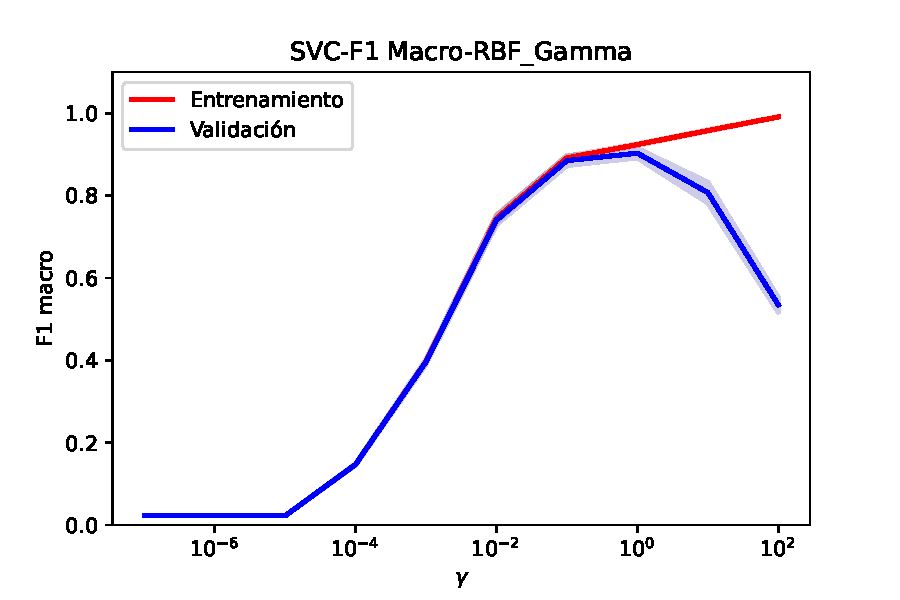
\includegraphics[width=\textwidth]{imagenes/resultados/svm/curvas_validacion/SVC-F1 Macro-RBF_Gamma.pdf}
	\caption{Curva de validación para kernel RBF en función de $\gamma$ en área C1c9.}
	\label{res:svc_vc_rbf_gamma}
\end{figure}

A partir de $\gamma = 10^{-2} = 0.01$ el modelo empieza a sobre ajustar los datos de entrenamiento frente a validación, divergiendo completamente a partir de $\gamma=10^{-1}=0.1$. Para $\gamma<10^{-2}$ el rendimiento para entrenamiento y validación muestran los mismos resultados, indicando que el modelo funciona correctamente para tal rango. Sin embargo, el rendimiento para estos valores es muy bajo.

\paragraph{Kernel polinómico}

Definido por la ecuación \ref{eqn:svm_kernel_poly}, el kernel polinómico es dependiente de parámetros $\gamma$, $r$ (también llamado \textit{coef0}) y $d$ (grado del polinomio, en inglés \textit{degree}).

\begin{figure}[H]
	\captionsetup{justification=centering}
	\centering
	\begin{subfigure}[b]{.45\linewidth}
		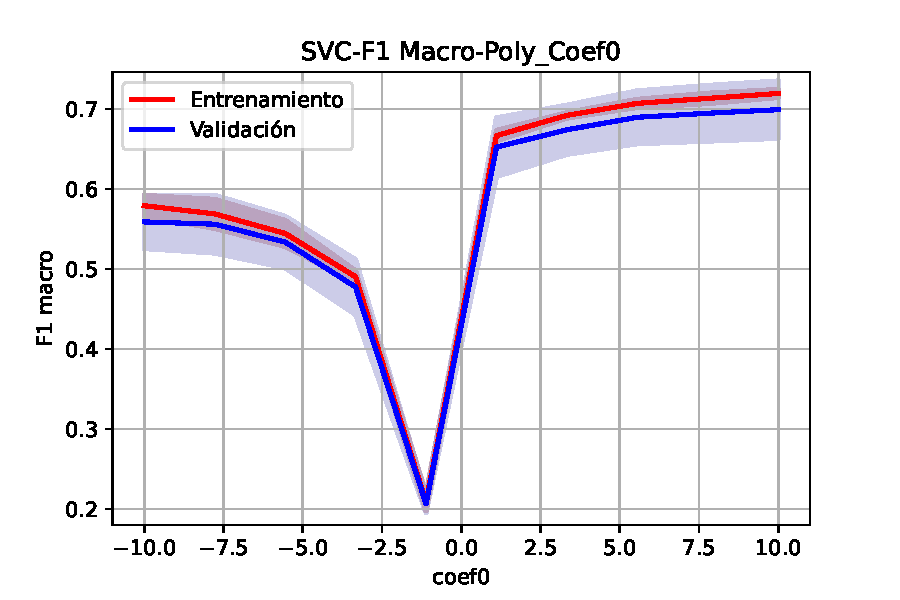
\includegraphics[width=\linewidth]{imagenes/resultados/svm/curvas_validacion/SVC-F1 Macro-Poly_Coef0.pdf}
		\caption{Curva de validación para kernel polinómico en función de $r$ en área C1c9.}
		\label{res:svc_vc_poly_coef0}
	\end{subfigure}
	\begin{subfigure}[b]{.45\linewidth}
		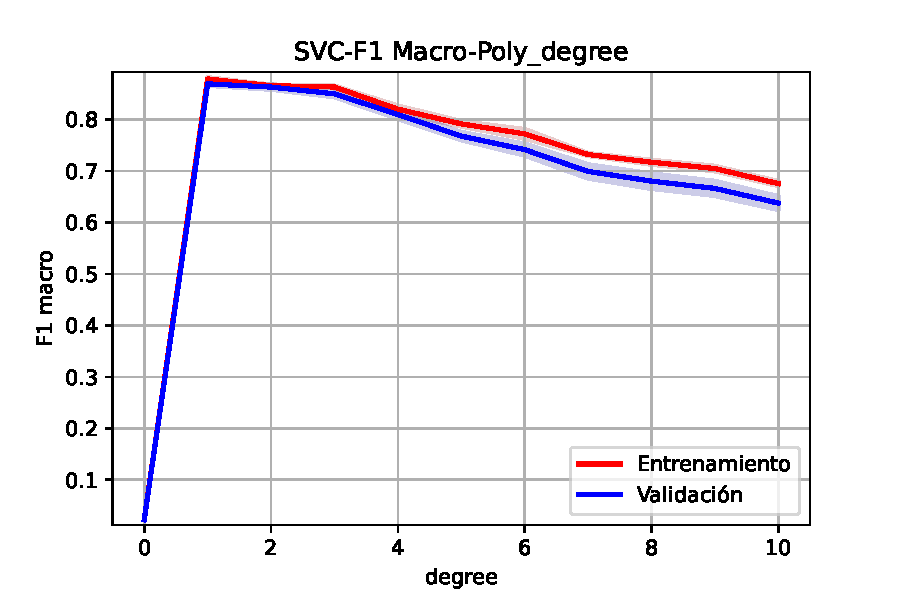
\includegraphics[width=\linewidth]{imagenes/resultados/svm/curvas_validacion/SVC-F1 Macro-Poly_degree.pdf}
		\caption{Curva de validación para kernel polinómico en función del grado en área C1c9.}
		\label{res:svc_vc_poly_degree}
	\end{subfigure}
	\caption{Curvas de validación para kernel polinómico}
	\label{res:svc_vc_poly_kernel}
\end{figure}

La figura \ref{res:svc_vc_poly_coef0} representa un correcto comportamiento del modelo para el rango $r\epsilon[-3,1.75]$, sobre ajustando fuera de estos límites. Para \ref{res:svc_vc_poly_degree}, el modelo funciona correctamente en $d<3$, tendiendo a sobre ajustar a medida que se aumenta el grado del kernel.

\paragraph{Kernel lineal}

El kernel lineal (ecuación \ref{eqn:svm_kernel_lineal}) no requiere de más parámetros excepto $C$, el parámetro de regularización, por lo tanto, su curva de validación ya se haya representada en \ref{res:svc_vc_lineal}.

\subsubsection{Mejores parámetros SVC para área C1C9}

\paragraph{Kernel RBF}

Los mejores parámetros encontrados, según métrica $F_{1}$, para $k\:(\mbox{ANOVA})\:\epsilon\:[2,31]$, $\gamma\:\epsilon\:[10^{-7},10^{2}]$ y $C\:\epsilon\:[1,100]$ han resultado:

\begin{table}[H]
	\begin{tabular}{|c|c|}
		\hline
		Parámetro & Valor \\ \hline
		k (ANOVA) & 9 \\ \hline
		C & 20\\ \hline
		$\gamma$ & 1\\ \hline
	\end{tabular}
\end{table}

\paragraph{Kernel Lineal}

Los mejores parámetros encontrados, según métrica $F_{1}$, para $k\:(\mbox{ANOVA})\:\epsilon\:[2,31]$ y $C\:\epsilon\:[1,100]$ han resultado:

\begin{table}[H]
	\begin{tabular}{|c|c|}
		\hline
		Parámetro & Valor \\ \hline
		k (ANOVA) & 9 \\ \hline
		C & 15\\ \hline
	\end{tabular}
\end{table}

\paragraph{Kernel polinómico}

Los mejores parámetros encontrados, según métrica $F_{1}$, para $k\:(\mbox{ANOVA})\:\epsilon\:[2,31]$ y $C\:\epsilon\:[1,100]$ han resultado:

\begin{table}[H]
	\begin{tabular}{|c|c|}
		\hline
		Parámetro & Valor \\ \hline
		k (ANOVA) & 9 \\ \hline
		C & 15\\ \hline
		r & 1 \\ \hline
		Grado & 3 \\ \hline
		$\gamma$ & 1 \\ \hline
	\end{tabular}
\end{table}

\begin{table}[H]
	\centering
	\captionsetup{justification=centering}
	\resizebox{\columnwidth}{!}{
	\begin{tabular}{|c|c|c|c|}
		\hline
		\multicolumn{2}{|c|}{AUC-Ovo-C1C9-Poly} \\ \hline \hline
		Clase & AUC \\ \hline
		LE06 & 0.897256 \\ \hline
		LE07 & 0.801268 \\ \hline
		LE09a & 1.000000 \\ \hline
		LE10 & 0.982807 \\ \hline
		LE11 & 0.898879 \\ \hline
		LE12 & 0.992003 \\ \hline
		LE13 & 0.943605 \\ \hline
		MO02 & 0.989694 \\ \hline
		MO05 & 0.999336 \\ \hline
		MO08 & 0.982773 \\ \hline
		MO10 & 0.999272 \\ \hline
		MO15 & 0.985674 \\ \hline
		MO17 & 0.988889 \\ \hline
		MO20 & 0.596893 \\ \hline
		MO22 & 0.997976 \\ \hline
	\end{tabular}
	\begin{tabular}{|c|c|}
		\hline
		\multicolumn{2}{|c|}{AUC-Ovo-C1C9-Lineal} \\ \hline \hline
		Clase & AUC \\ \hline
		LE06 & 0.835289 \\ \hline
		LE07 & 0.703032 \\ \hline
		LE09a & 1.000000 \\ \hline
		LE10 & 0.972459 \\ \hline
		LE11 & 0.863337 \\ \hline
		LE12 & 0.924740 \\ \hline
		LE13 & 0.776634 \\ \hline
		MO02 & 0.990316 \\ \hline
		MO05 & 0.999177 \\ \hline
		MO08 & 0.955717 \\ \hline
		MO10 & 0.999730 \\ \hline
		MO15 & 0.966846 \\ \hline
		MO17 & 1.000000 \\ \hline
		MO20 & 0.667409 \\ \hline
		MO22 & 0.996742 \\ \hline
	\end{tabular}
	\begin{tabular}{|c|c|}
		\hline
		\multicolumn{2}{|c|}{AUC-Ovo-C1C9-RBF} \\ \hline \hline
		Clase & AUC \\ \hline
		LE06 & 0.923290 \\ \hline
		LE07 & 0.797598 \\ \hline
		LE09a & 1.000000 \\ \hline
		LE10 & 0.986225 \\ \hline
		LE11 & 0.934888 \\ \hline
		LE12 & 0.990411 \\ \hline
		LE13 & 0.943534 \\ \hline
		MO02 & 0.997832 \\ \hline
		MO05 & 0.998750 \\ \hline
		MO08 & 0.992643 \\ \hline
		MO10 & 0.999781 \\ \hline
		MO15 & 0.993808 \\ \hline
		MO17 & 0.979798 \\ \hline
		MO20 & 0.646762 \\ \hline
		MO22 & 0.997654 \\ \hline
	\end{tabular}}
	\caption{Resultados AUC para diferentes Kernel SVM para área C1C9}
	\label{res:svc_c1c9}
\end{table}

\begin{table}[H]
	\centering
	\captionsetup{justification=centering}
	\begin{tabular}{|c|c|}
		\hline
		Kernel & AUC Macro \\ \hline \hline
		Polinómico & 0.9371 \\ \hline
		Lineal & 0.9116 \\ \hline
		RBF & 0.9467 \\ \hline
	\end{tabular}
	\caption{AUC macro para C1C9}
	\label{res:svc_auc_macro_c1c9}	
\end{table}

\subsection{SVM con área B345}

\subsubsection{Curvas de validación para diferentes Kernel}

La cuadrícula de imágenes \ref{res:svc_vc_b345} representa las curvas de validación para los diferentes kernel aplicables a un modelo SVM, implementados en la clase SVC de \textit{Sklearn}, definidos en las ecuaciones \ref{eqn:svm_kernel_lineal}, \ref{eqn:svm_kernel_rbf}, \ref{eqn:svm_kernel_poly} y \ref{eqn:svm_kernel_sigmoid}.

\begin{figure}[H]
	\captionsetup{justification=centering}
	\centering
	\begin{subfigure}[b]{.45\linewidth}
		\includegraphics[width=\linewidth]{imagenes/resultados/svm/curvas_validacion/b345/SVC-F1 Macro-linear_C.pdf}
		\caption{Kernel Lineal}
		\label{res:svc_vc_lineal_b345}
	\end{subfigure}
	\begin{subfigure}[b]{.45\linewidth}
		\includegraphics[width=\linewidth]{imagenes/resultados/svm/curvas_validacion/b345/SVC-F1 Macro-poly_C.pdf}
		\caption{Kernel polinómico}
		\label{res:svc_vc_poly_b345}
	\end{subfigure}
	\begin{subfigure}[b]{.45\linewidth}
		\includegraphics[width=\linewidth]{imagenes/resultados/svm/curvas_validacion/b345/SVC-F1 Macro-rbf_C.pdf}
		\caption{Kernel RBF}
		\label{res:svc_vc_rbf_b345}
	\end{subfigure}
	\begin{subfigure}[b]{.45\linewidth}
		\includegraphics[width=\linewidth]{imagenes/resultados/svm/curvas_validacion/b345/SVC-F1 Macro-sigmoid_C.pdf}
		\caption{Kernel Sigmoid}
		\label{res:svc_vc_sigmoid_b345}
	\end{subfigure}
	\caption{Curvas de validación para kernels de modelo SVC en área B345 en función de parámetro de penalización C.}
	\label{res:svc_vc_b345}
\end{figure}

Para los cuatro kernel disponibles en la clase SVC de \textit{Sklearn}, en general, el modelo presenta obreajuste de los datos de entrenamiento frente a los de validación. La figura \ref{res:svc_vc_sigmoid} presenta un rendimiento inferior a 0.5, indicando que el kernel \textit{sigmoid} no es aplicable a esta clasificación.

\paragraph{Kernel RBF}

El kernel RBF (ecuación \ref{eqn:svm_kernel_rbf}) depende del parámetro $\gamma$ en su definición. La figura \ref{res:svc_vc_rbf_gamma_b345} representa la curva de validación de dicho parámetro:

\begin{figure}[H]
	\centering
	\captionsetup{justification=centering}
	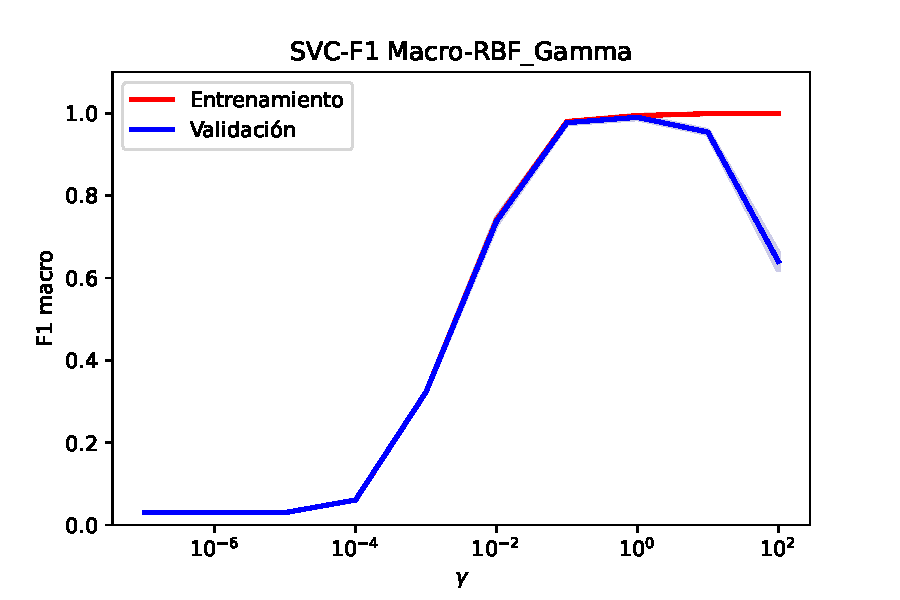
\includegraphics[width=\textwidth]{imagenes/resultados/svm/curvas_validacion/b345/SVC-F1 Macro-RBF_Gamma.pdf}
	\caption{Curva de validación para kernel RBF en función de $\gamma$ en área B345.}
	\label{res:svc_vc_rbf_gamma_b345}
\end{figure}

El modelo presenta un comportamiento perfecto para $\gamma<10^{-1}$, sobre ajustando para valores superiores.

\paragraph{Kernel polinómico}

Definido por la ecuación \ref{eqn:svm_kernel_poly}, el kernel polinómico es dependiente de parámetros $\gamma$, $r$ (también llamado \textit{coef0}) y $d$ (grado del polinomio, en inglés \textit{degree}).

\begin{figure}[H]
	\captionsetup{justification=centering}
	\centering
	\begin{subfigure}[b]{.45\linewidth}
		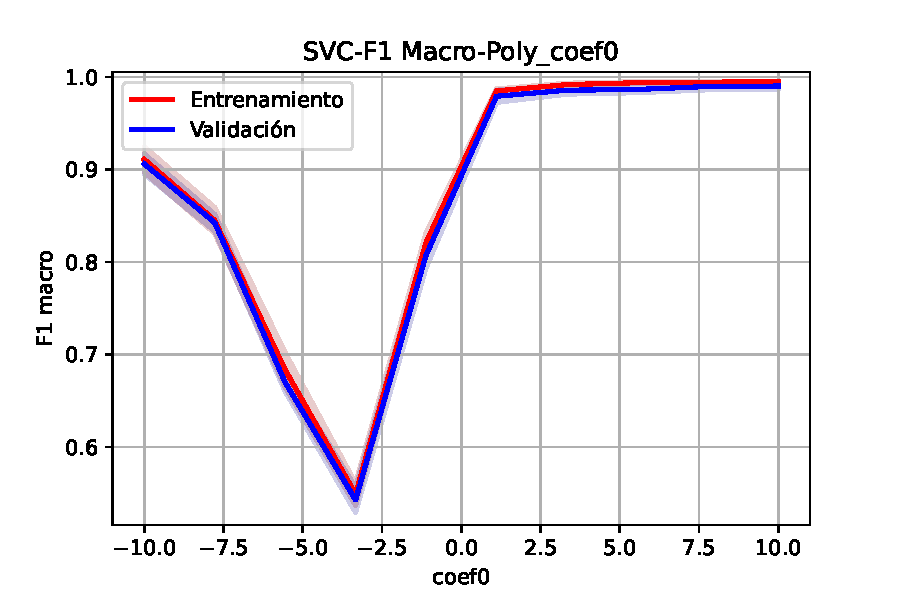
\includegraphics[width=\linewidth]{imagenes/resultados/svm/curvas_validacion/b345/SVC-F1 Macro-Poly_coef0.pdf}
		\caption{Curva de validación para kernel polinómico en función de $r$ en área B345.}
		\label{res:svc_vc_poly_coef0_b345}
	\end{subfigure}
	\begin{subfigure}[b]{.45\linewidth}
		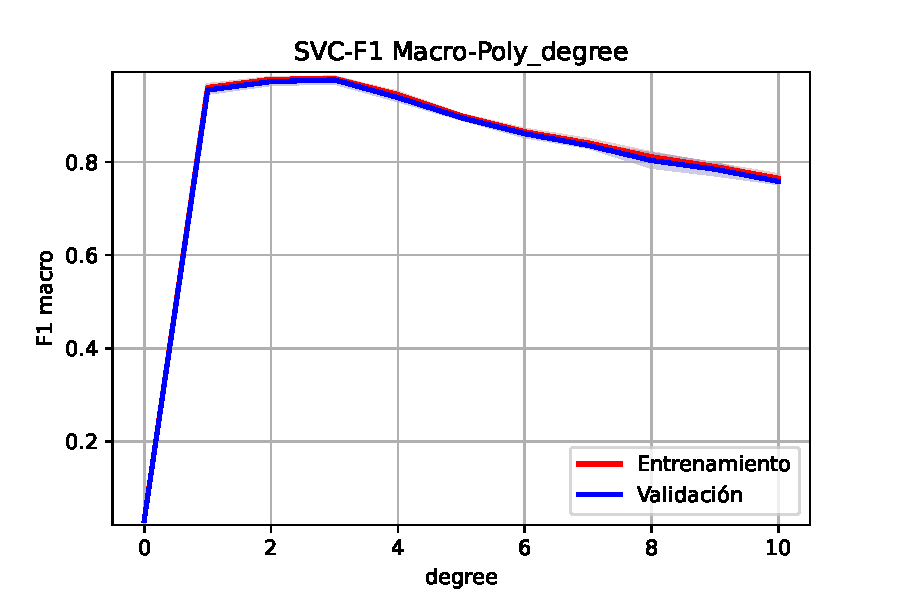
\includegraphics[width=\linewidth]{imagenes/resultados/svm/curvas_validacion/b345/SVC-F1 Macro-Poly_degree.pdf}
		\caption{Curva de validación para kernel polinómico en función del grado en área B345.}
		\label{res:svc_vc_poly_degree_b345}
	\end{subfigure}
	\caption{Curvas de validación para kernel polinómico}
	\label{res:svc_vc_poly_kernel_b345}
\end{figure}

Para el caso del parámetro $r$, el modelo sobre ajusta en casi todo el rango, pero es de tan mínima la diferencia que se puede considerar un comportamiento casi perfecto. En el caso de $d$, el clasificador es impecable pues, ni sobre ajusta ni sub ajusta.

La figura \ref{res:svc_vc_poly_coef0_b345} representa un correcto comportamiento del modelo para el rango $r\epsilon[-3,1.75]$, sobre ajustando fuera de estos límites. Para \ref{res:svc_vc_poly_degree_b345}, el modelo funciona correctamente en $d<3$, tendiendo a sobre ajustar a medida que se aumenta el grado del kernel.

\paragraph{Kernel lineal}

El kernel lineal (ecuación \ref{eqn:svm_kernel_lineal}) no requiere de más parámetros excepto $C$, el parámetro de regularización, por lo tanto, su curva de validación ya se haya representada en \ref{res:svc_vc_lineal_b345}.

\subsubsection{Mejores parámetros SVC para área B345}

\paragraph{Kernel RBF}

Los mejores parámetros encontrados, según métrica $F_{1}$, para $k\:(\mbox{ANOVA})\:\epsilon\:[2,31]$, $\gamma\:\epsilon\:[10^{-7},10^{-1}]$ y $C\:\epsilon\:[1,100]$ han resultado:

\begin{table}[H]
	\begin{tabular}{|c|c|}
		\hline
		Parámetro & Valor \\ \hline
		k (ANOVA) & 12 \\ \hline
		C & 20\\ \hline
		$\gamma$ & 0.1\\ \hline
	\end{tabular}
\end{table}

\paragraph{Kernel Lineal}

Los mejores parámetros encontrados, según métrica $F_{1}$, para $k\:(\mbox{ANOVA})\:\epsilon\:[2,31]$ y $C\:\epsilon\:[1,100]$ han resultado:

\begin{table}[H]
	\begin{tabular}{|c|c|}
		\hline
		Parámetro & Valor \\ \hline
		k (ANOVA) & 12 \\ \hline
		C & 15\\ \hline
	\end{tabular}
\end{table}

\paragraph{Kernel polinómico}

Los mejores parámetros encontrados, según métrica $F_{1}$, para $k\:(\mbox{ANOVA})\:\epsilon\:[2,31]$ y $C\:\epsilon\:[1,100]$ han resultado:

\begin{table}[H]
	\begin{tabular}{|c|c|}
		\hline
		Parámetro & Valor \\ \hline
		k (ANOVA) & 12 \\ \hline
		C & 20\\ \hline
		r & 1 \\ \hline
		Grado & 3 \\ \hline
		$\gamma$ & 1 \\ \hline
	\end{tabular}
\end{table}

\begin{table}[H]
	\centering
	\captionsetup{justification=centering}
	\resizebox{\columnwidth}{!}{
		\begin{tabular}{|c|c|c|c|}
			\hline
			\multicolumn{2}{|c|}{AUC-Ovo-B345-Poly} \\ \hline \hline
			Clase & AUC \\ \hline
			LX01 & 1.000000 \\ \hline
			TC01 & 1.000000 \\ \hline
			TC02 & 1.000000 \\ \hline
			TC03 & 1.000000 \\ \hline
			TC04 & 1.000000 \\ \hline
			TC05 & 1.000000 \\ \hline
			TC06 & 1.000000 \\ \hline
			TC08 & 1.000000 \\ \hline
			TC10 & 0.982638 \\ \hline
			TC11 & 0.996768 \\ \hline
			TC12 & 1.000000 \\ \hline
			TC14 & 1.000000 \\ \hline
			TC15 & 1.000000 \\ \hline
			TC17 & 0.993755 \\ \hline
			TC19 & 1.000000 \\ \hline
			TC20 & 1.000000 \\ \hline
			TC23 & 1.000000 \\ \hline
			TC25 & 1.000000 \\ \hline
			TC27 & 1.000000 \\ \hline
			TC29 & 1.000000 \\ \hline
			TC31 & 1.000000 \\ \hline
			TC35 & 1.000000 \\ \hline
		\end{tabular}
		\begin{tabular}{|c|c|}
			\hline
			\multicolumn{2}{|c|}{AUC-Ovo-B345-Lineal} \\ \hline \hline
			Clase & AUC \\ \hline
			LX01 & 1.000000 \\ \hline
			TC01 & 1.000000 \\ \hline
			TC02 & 1.000000 \\ \hline
			TC03 & 1.000000 \\ \hline
			TC04 & 1.000000 \\ \hline
			TC05 & 1.000000 \\ \hline
			TC06 & 1.000000 \\ \hline
			TC08 & 1.000000 \\ \hline
			TC10 & 0.765972 \\ \hline
			TC11 & 0.963289 \\ \hline
			TC12 & 1.000000 \\ \hline
			TC14 & 1.000000 \\ \hline
			TC15 & 1.000000 \\ \hline
			TC17 & 0.999905 \\ \hline
			TC19 & 1.000000 \\ \hline
			TC20 & 1.000000 \\ \hline
			TC23 & 1.000000 \\ \hline
			TC25 & 1.000000 \\ \hline
			TC27 & 1.000000 \\ \hline
			TC29 & 1.000000 \\ \hline
			TC31 & 1.000000 \\ \hline
			TC35 & 1.000000 \\ \hline
		\end{tabular}
		\begin{tabular}{|c|c|}
			\hline
			\multicolumn{2}{|c|}{AUC-Ovo-B345-RBF} \\ \hline \hline
			Clase & AUC \\ \hline
			LX01 & 1.000000 \\ \hline
			TC01 & 1.000000 \\ \hline
			TC02 & 1.000000 \\ \hline
			TC03 & 1.000000 \\ \hline
			TC04 & 1.000000 \\ \hline
			TC05 & 1.000000 \\ \hline
			TC06 & 1.000000 \\ \hline
			TC08 & 1.000000 \\ \hline
			TC10 & 0.971630 \\ \hline
			TC11 & 0.993925 \\ \hline
			TC12 & 1.000000 \\ \hline
			TC14 & 1.000000 \\ \hline
			TC15 & 1.000000 \\ \hline
			TC17 & 0.999905 \\ \hline
			TC19 & 1.000000 \\ \hline
			TC20 & 1.000000 \\ \hline
			TC23 & 1.000000 \\ \hline
			TC25 & 1.000000 \\ \hline
			TC27 & 1.000000 \\ \hline
			TC29 & 1.000000 \\ \hline
			TC31 & 1.000000 \\ \hline
			TC35 & 1.000000 \\ \hline
	\end{tabular}}
	\caption{Resultados AUC para diferentes Kernel SVM para área B345}
	\label{res:svc_b345}
\end{table}

\begin{table}[H]
	\centering
	\captionsetup{justification=centering}
	\begin{tabular}{|c|c|}
		\hline
		Kernel & AUC Macro \\ \hline \hline
		Polinómico & 0.9988 \\ \hline
		Lineal & 0.9877 \\ \hline
		RBF & 0.9984 \\ \hline
	\end{tabular}
	\caption{AUC macro para B345}
	\label{res:svc_auc_macro_b345}	
\end{table}


 %% NO AÑADIR %%
\input{conclusiones.tex}

% Los anexos pueden ir en la misma carpeta que el cuerpo del documento 
% porque eso facilita la migración de partes de un capítulo a un anexo.
\appendix\cleardoublepage
\hypertarget{ch:anexos}{%
    %----------
%	ANEXOS
%----------	

% Si tu trabajo incluye anexos, puedes descomentar las siguientes líneas
%\chapter* {Anexo x}
%\pagenumbering{gobble} % Las páginas de los anexos no se numeran}
    %\input{latex.tex}}

% La bibliografía no suele ir numerada porque se pone después de los anexos.
% No se debe poner antes de los anexos porque si se cita una referencia en
% un anexo sería una backward reference, que deben evitarse a toda costa
\cleardoublepage
\hypertarget{ch:bibliografia}{
    \printbibliography[heading=bibintoc,title={Bibliografía}]}
\cleardoublepage

\end{document}